\normalsize{ \indent
Para poder realizar lo propuesto, se ha utilizado una
máquina virtual; con objetivo de poder trasportar los
logros a distintas computadoras, además de evitar una
instalación fisica en hardware directamente. El
virtualizador que se ocupará es \acrshort{vmm},
considerando la facilidad que provee de personalización;
incluyendo características esenciales como traspaso de
dispositivos huésped y lector de discos, entre otros.
}
\newline
\normalsize{ \indent
Las características de los sistemas operativos
utilizados son:
}
\begin{figure}[!ht]
  \caption{Computadora huésped}
  \centering
  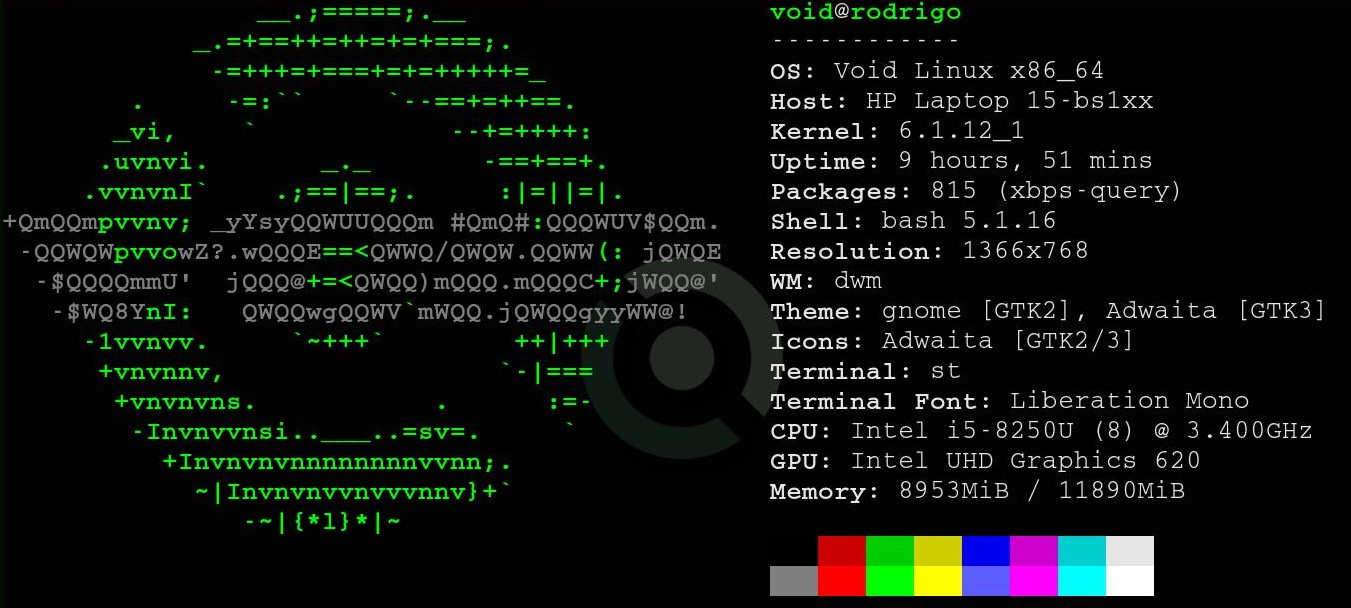
\includegraphics[width=\textwidth]{hostMachine}
\end{figure}
\begin{figure}[!ht]
  \caption{Máquina virtual}
  \centering
  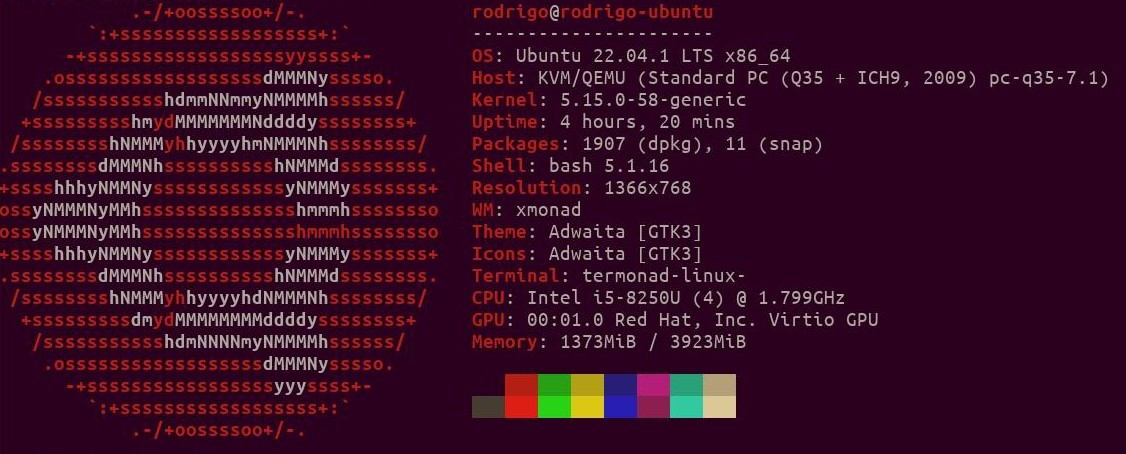
\includegraphics[width=\textwidth]{guestMachine}
\end{figure}
\newline
\normalsize{ \indent
La \acrlong{mv} se encuentra configurada de la
siguiente forma:
}
\newpage
\begin{figure}[!ht]
  \caption{Vistazo de \acrshort{mv}}
  \centering
  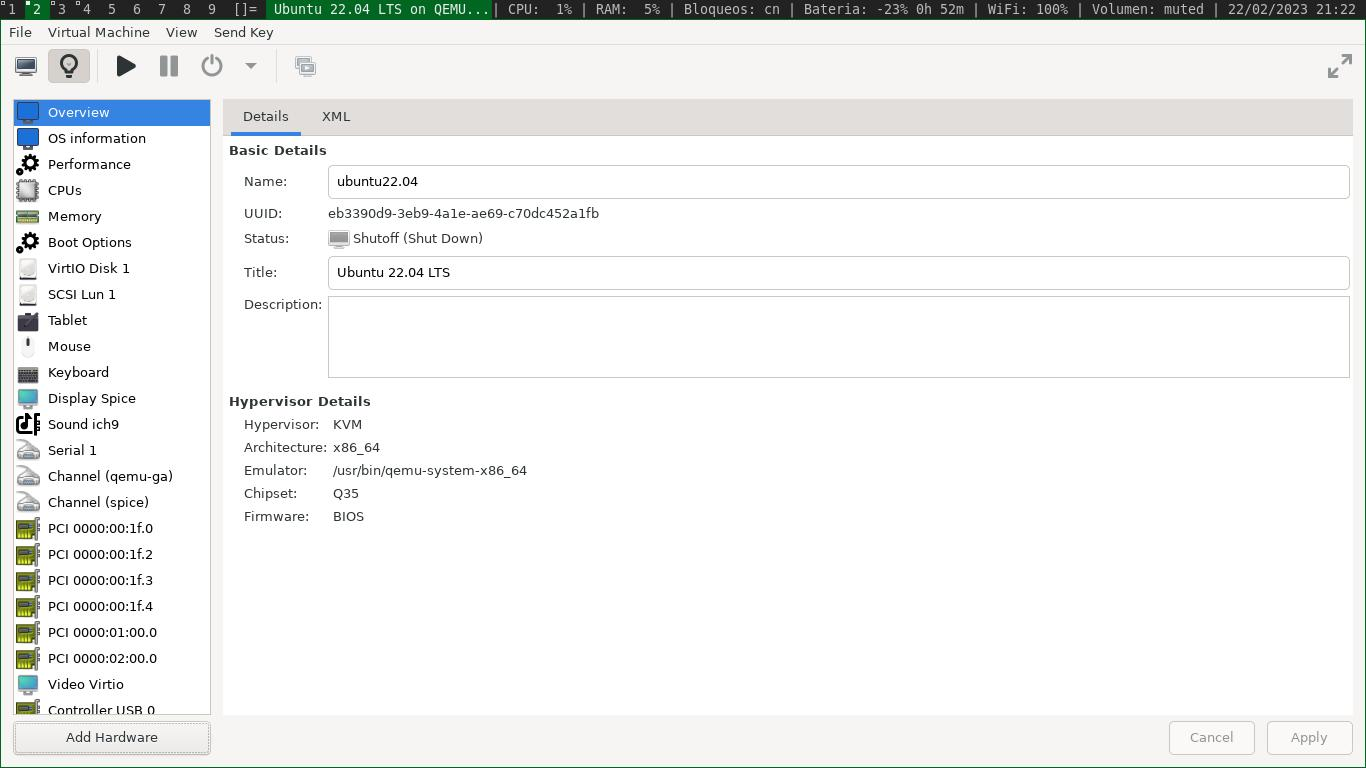
\includegraphics[width=\textwidth]{virtualMachine01}
\end{figure}
\begin{figure}[!ht]
  \caption{Información de \acrshort{so} de \acrshort{mv}}
  \centering
  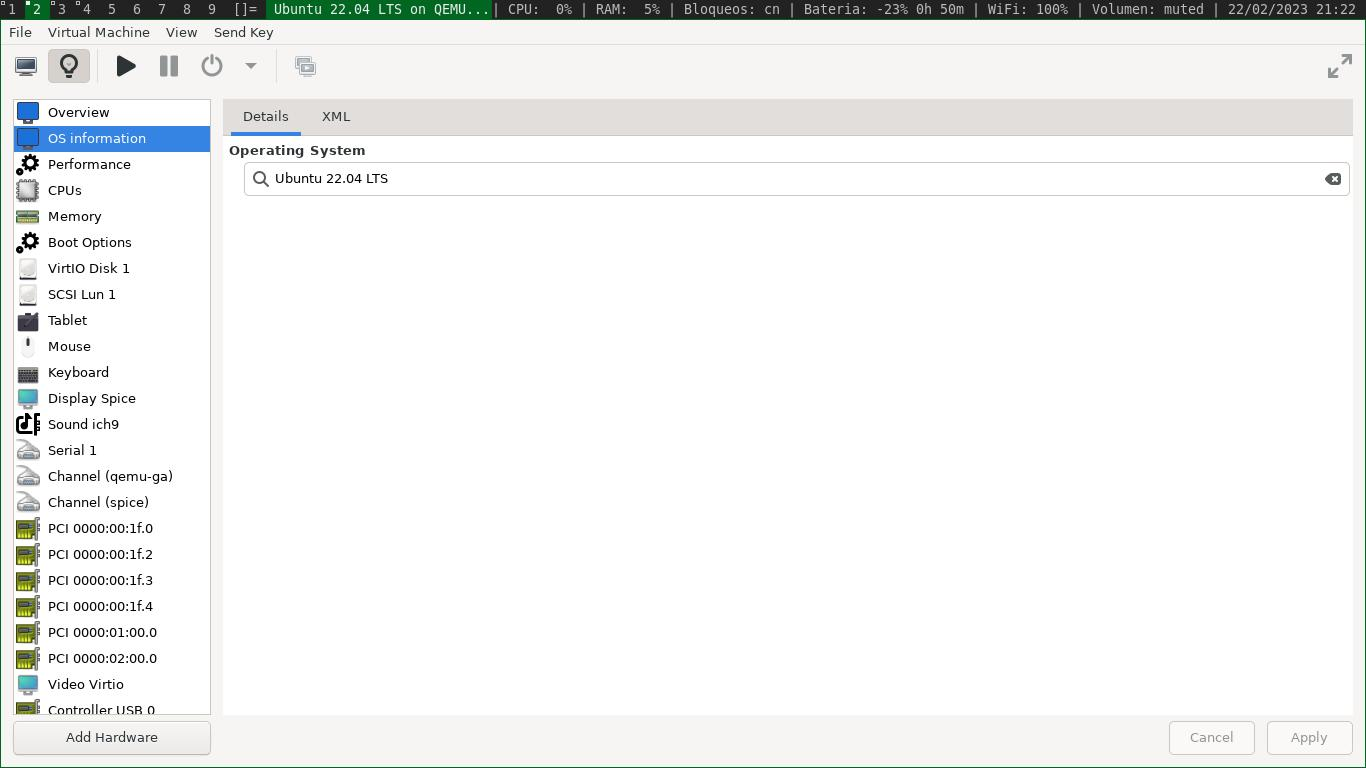
\includegraphics[width=\textwidth]{virtualMachine02}
\end{figure}
\newpage
\begin{figure}[!ht]
  \caption{\acrshort{cpu}s de \acrshort{mv}}
  \centering
  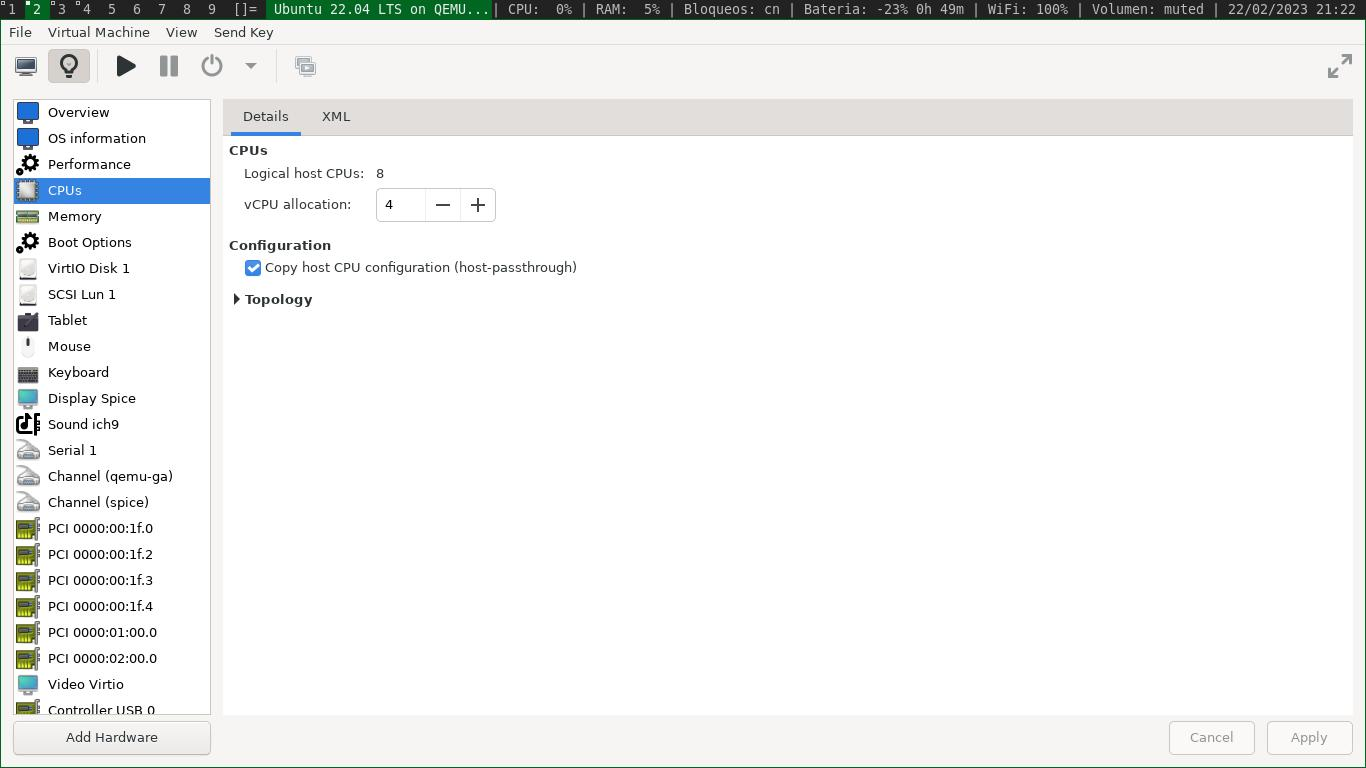
\includegraphics[width=\textwidth]{virtualMachine03}
\end{figure}
\begin{figure}[!ht]
  \caption{Memoria de \acrshort{mv}}
  \centering
  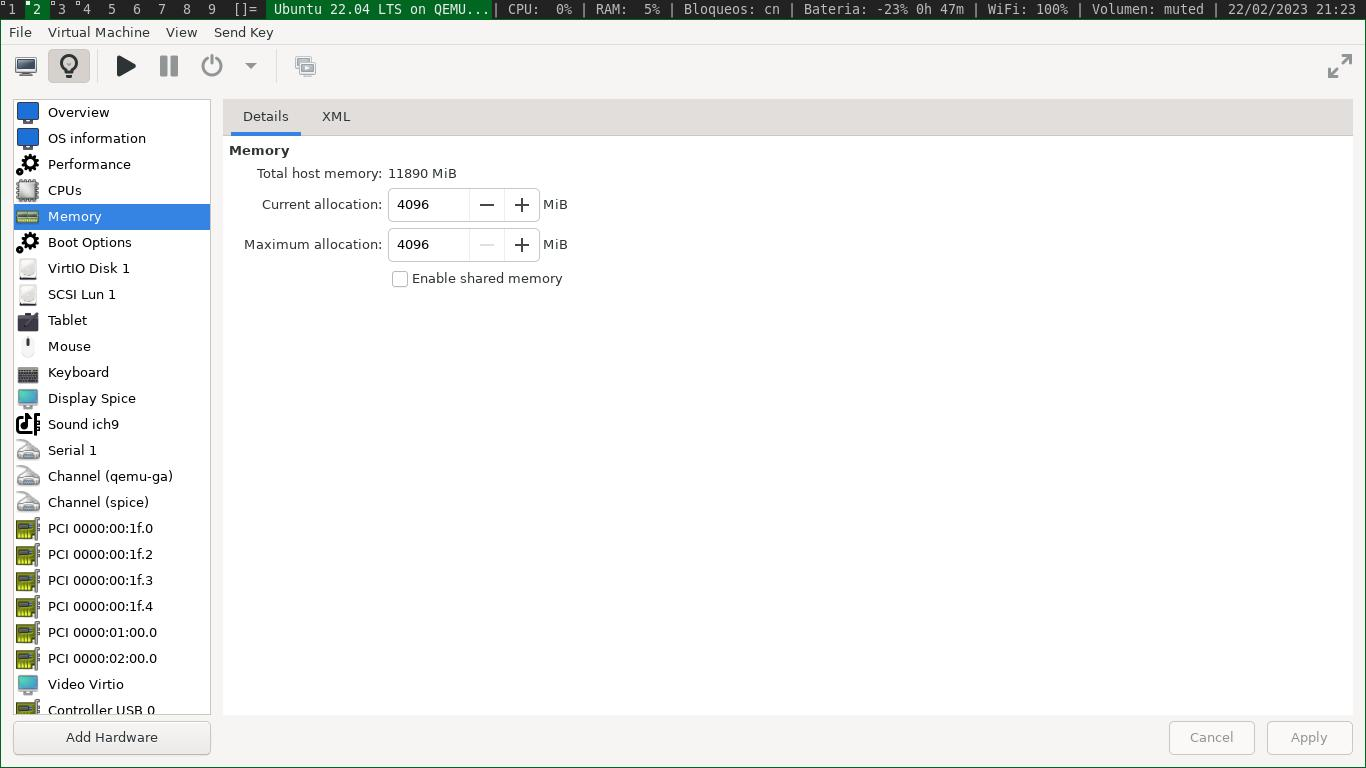
\includegraphics[width=\textwidth]{virtualMachine04}
\end{figure}
\newpage
\begin{figure}[!ht]
  \caption{Opciones de arranque de \acrshort{mv}}
  \centering
  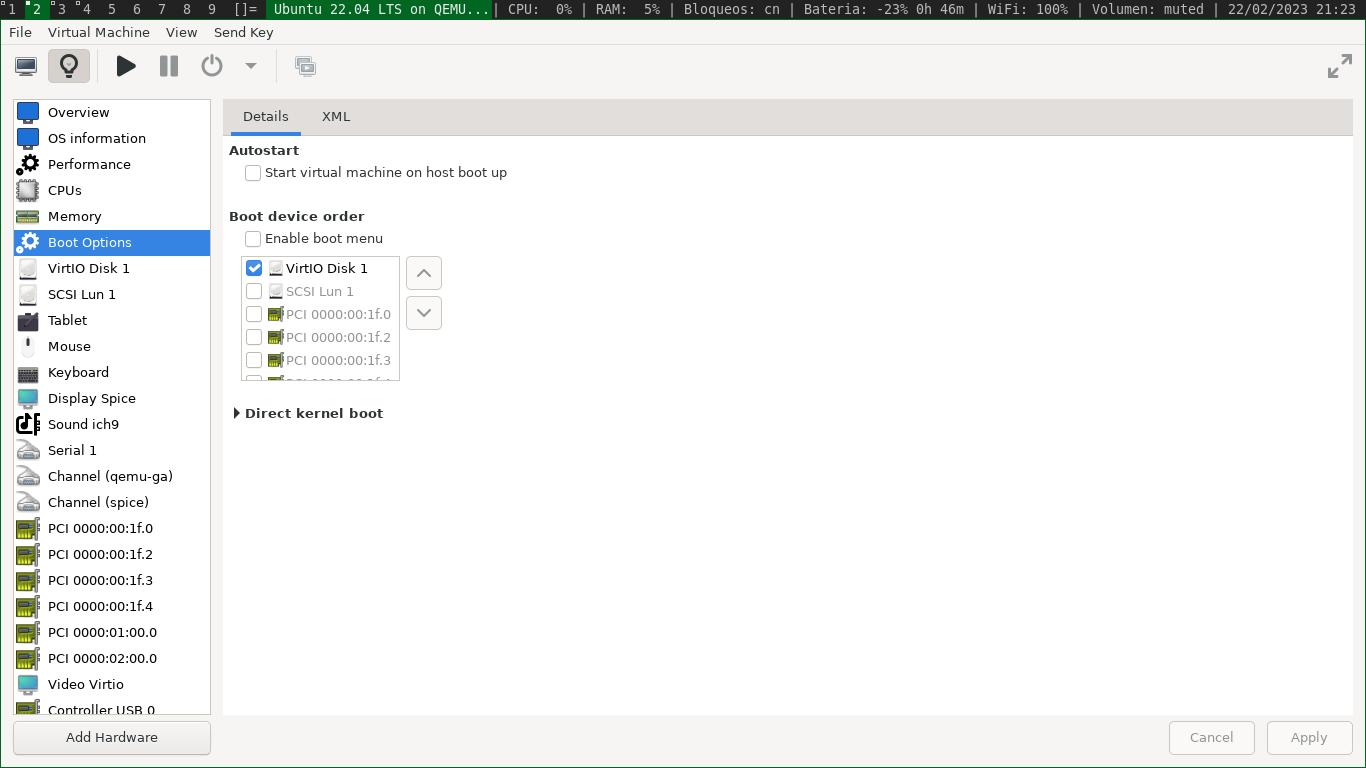
\includegraphics[width=\textwidth]{virtualMachine05}
\end{figure}
\begin{figure}[!ht]
  \caption{Disco VirtIO de \acrshort{mv}}
  \centering
  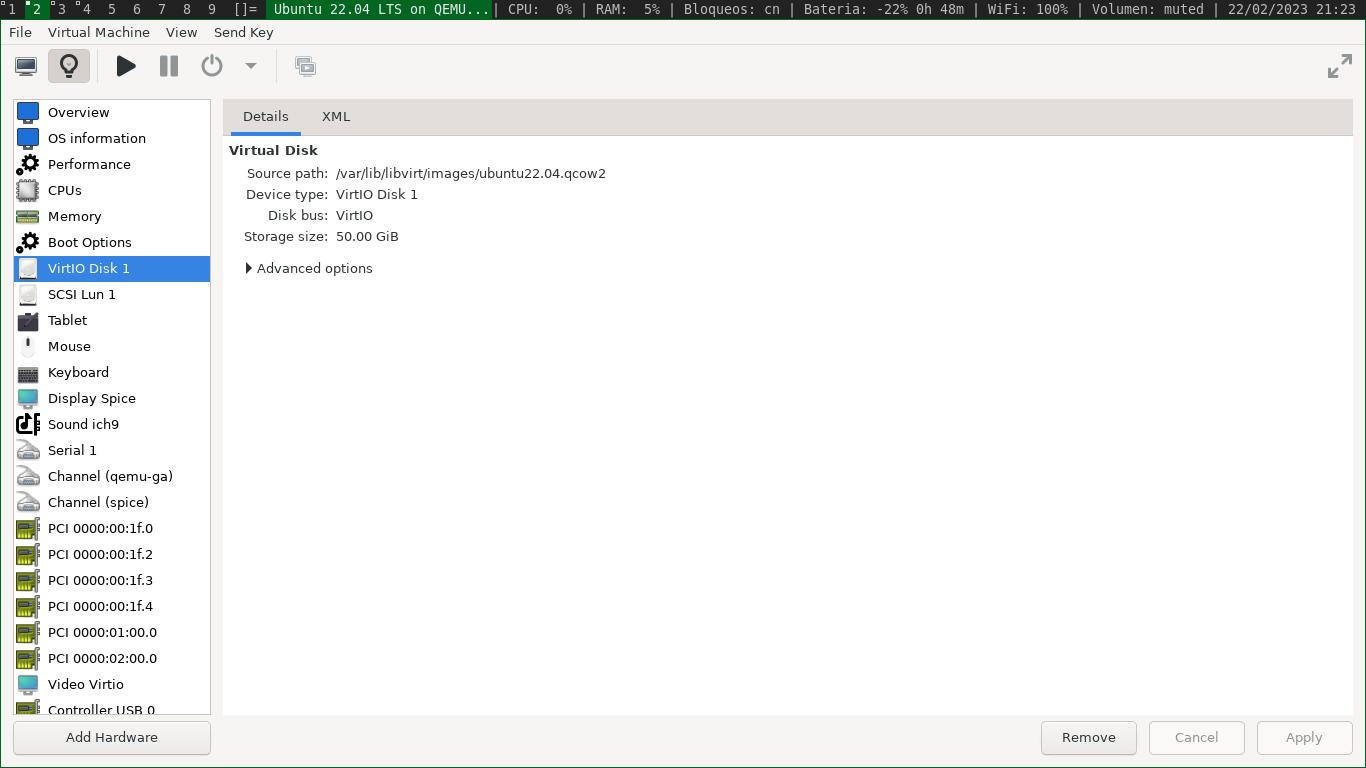
\includegraphics[width=\textwidth]{virtualMachine06}
\end{figure}
\newpage
\begin{figure}[!ht]
  \caption{Lector de discos en \acrshort{mv}}
  \centering
  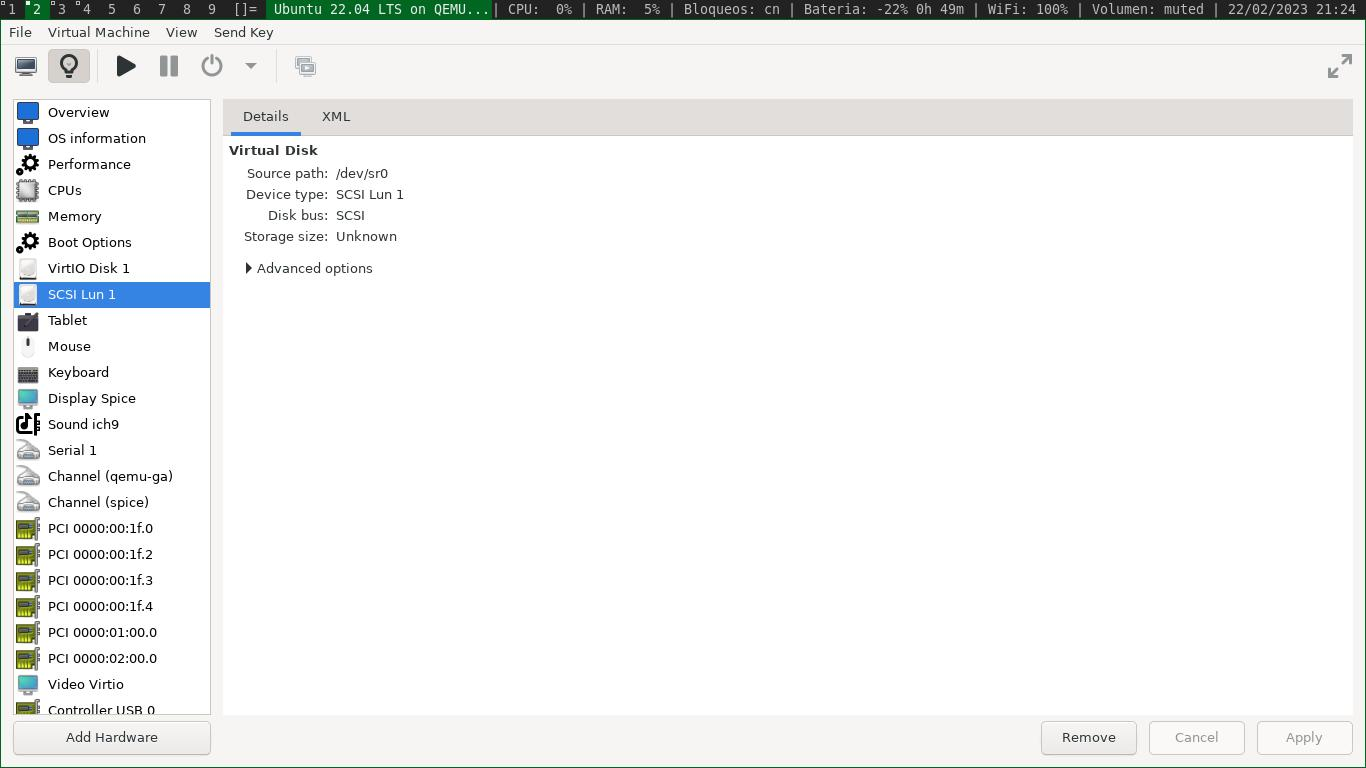
\includegraphics[width=\textwidth]{virtualMachine07}
\end{figure}
\begin{figure}[!ht]
  \caption{Tableta de \acrshort{mv}}
  \centering
  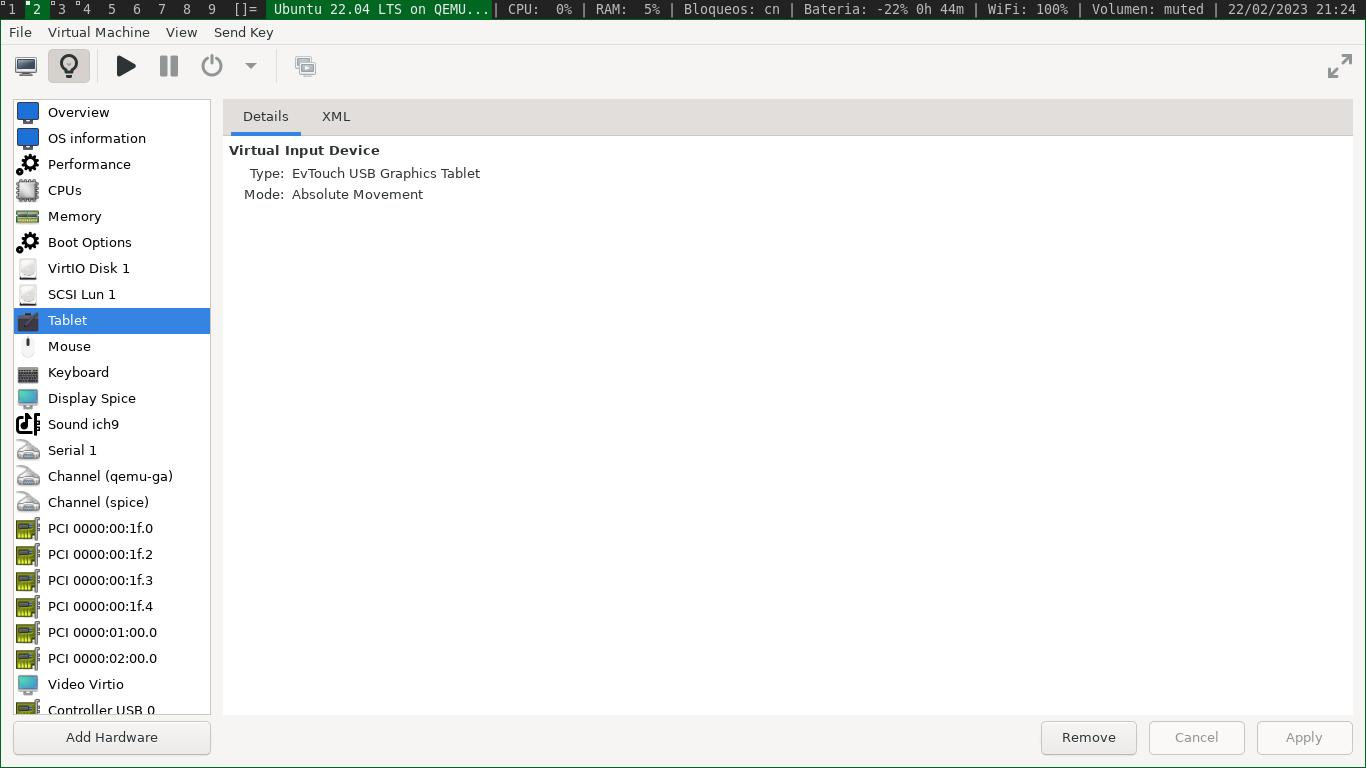
\includegraphics[width=\textwidth]{virtualMachine08}
\end{figure}
\newpage
\begin{figure}[!ht]
  \caption{Ratón de \acrshort{mv}}
  \centering
  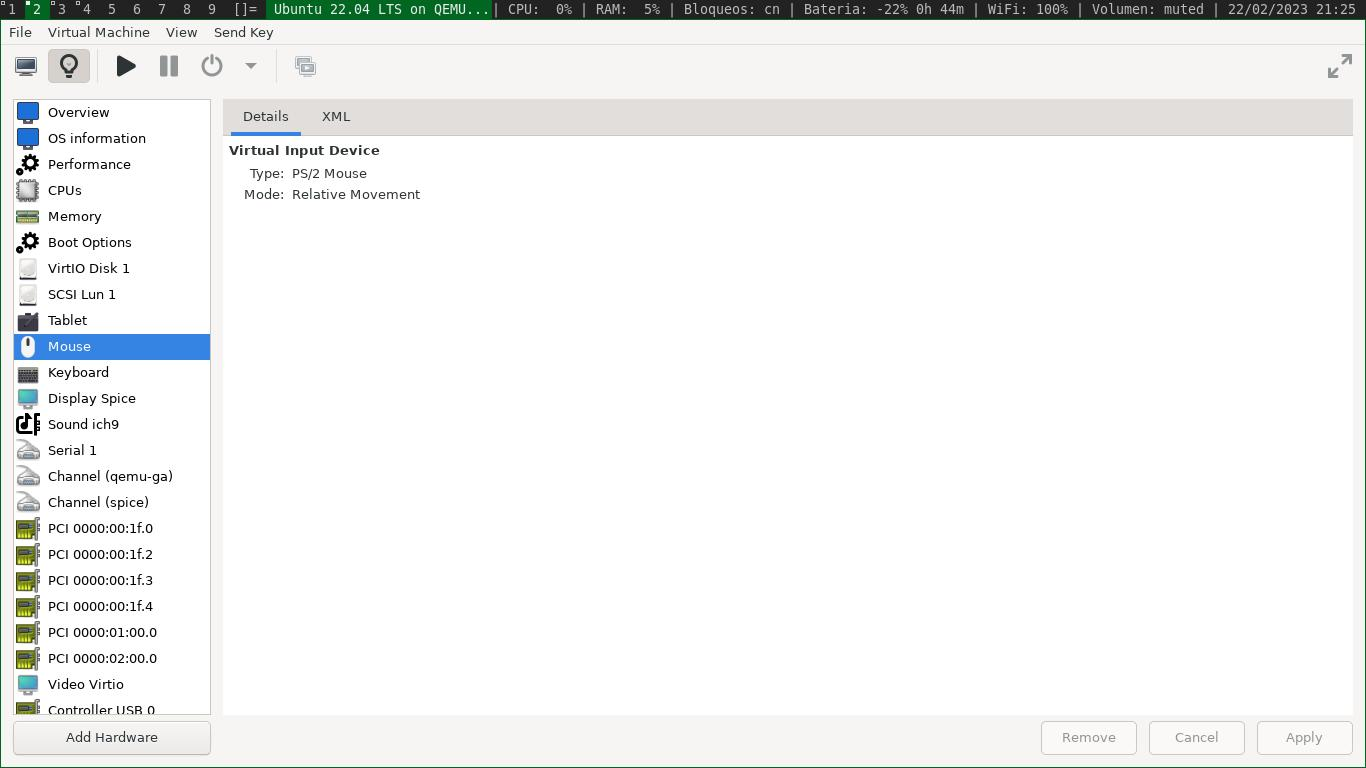
\includegraphics[width=\textwidth]{virtualMachine09}
\end{figure}
\begin{figure}[!ht]
  \caption{Teclado de \acrshort{mv}}
  \centering
  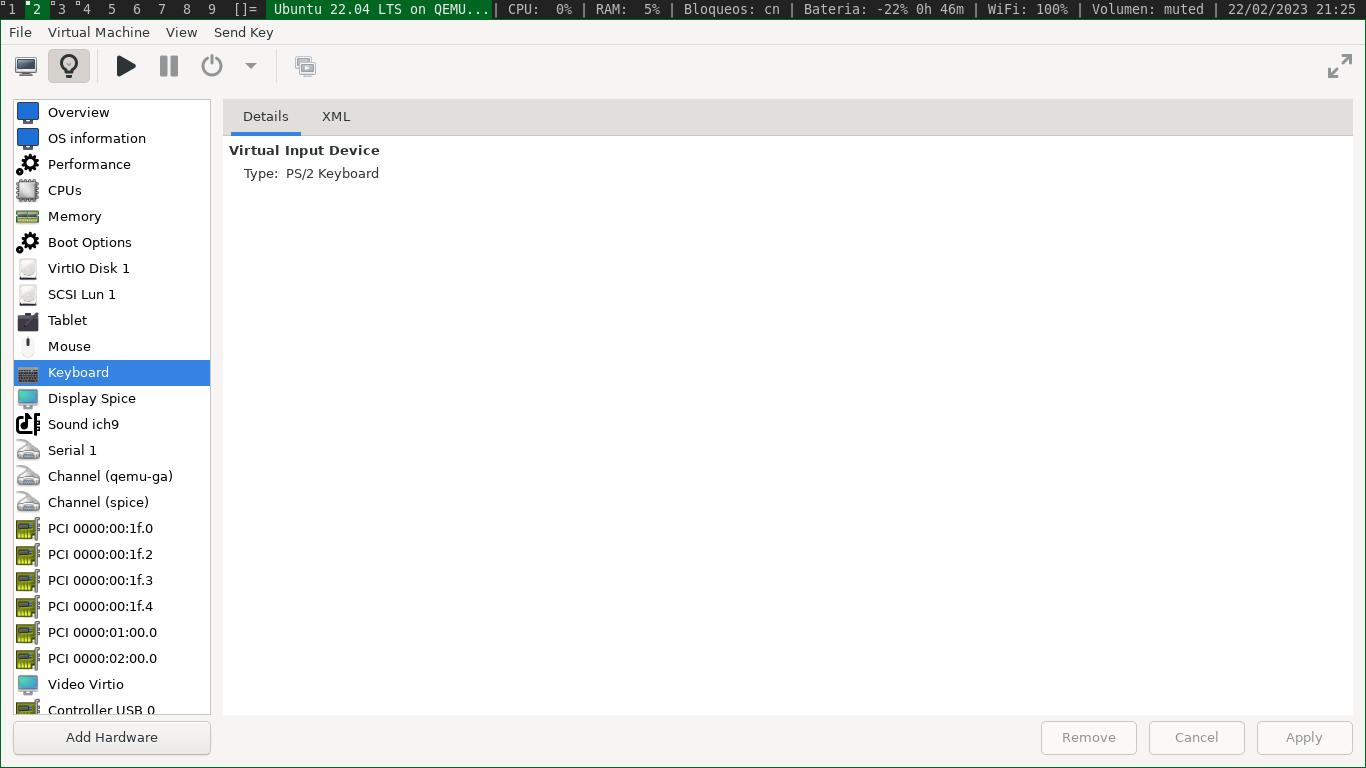
\includegraphics[width=\textwidth]{virtualMachine10}
\end{figure}
\newpage
\begin{figure}[!ht]
  \caption{Servidor de pantalla de \acrshort{mv}}
  \centering
  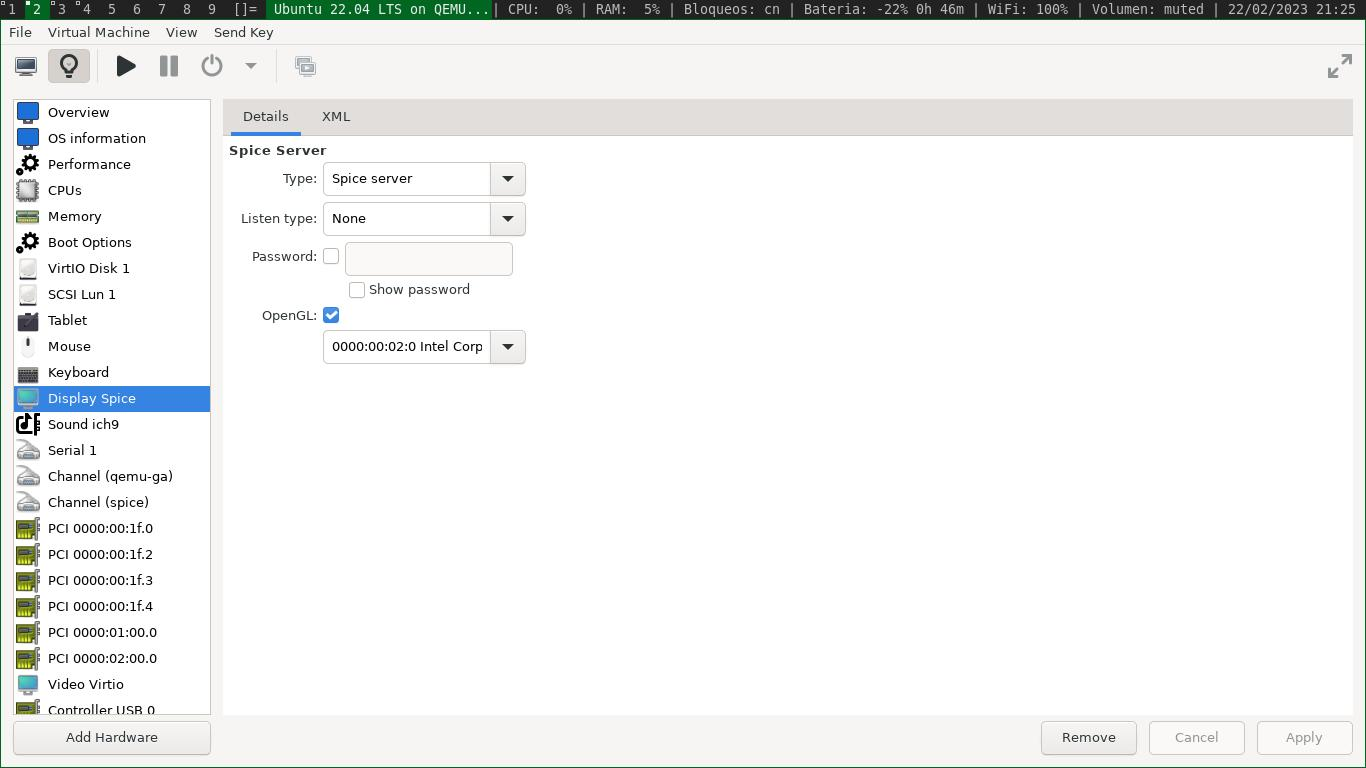
\includegraphics[width=\textwidth]{virtualMachine11}
\end{figure}
\begin{figure}[!ht]
  \caption{Sonido de \acrshort{mv}}
  \centering
  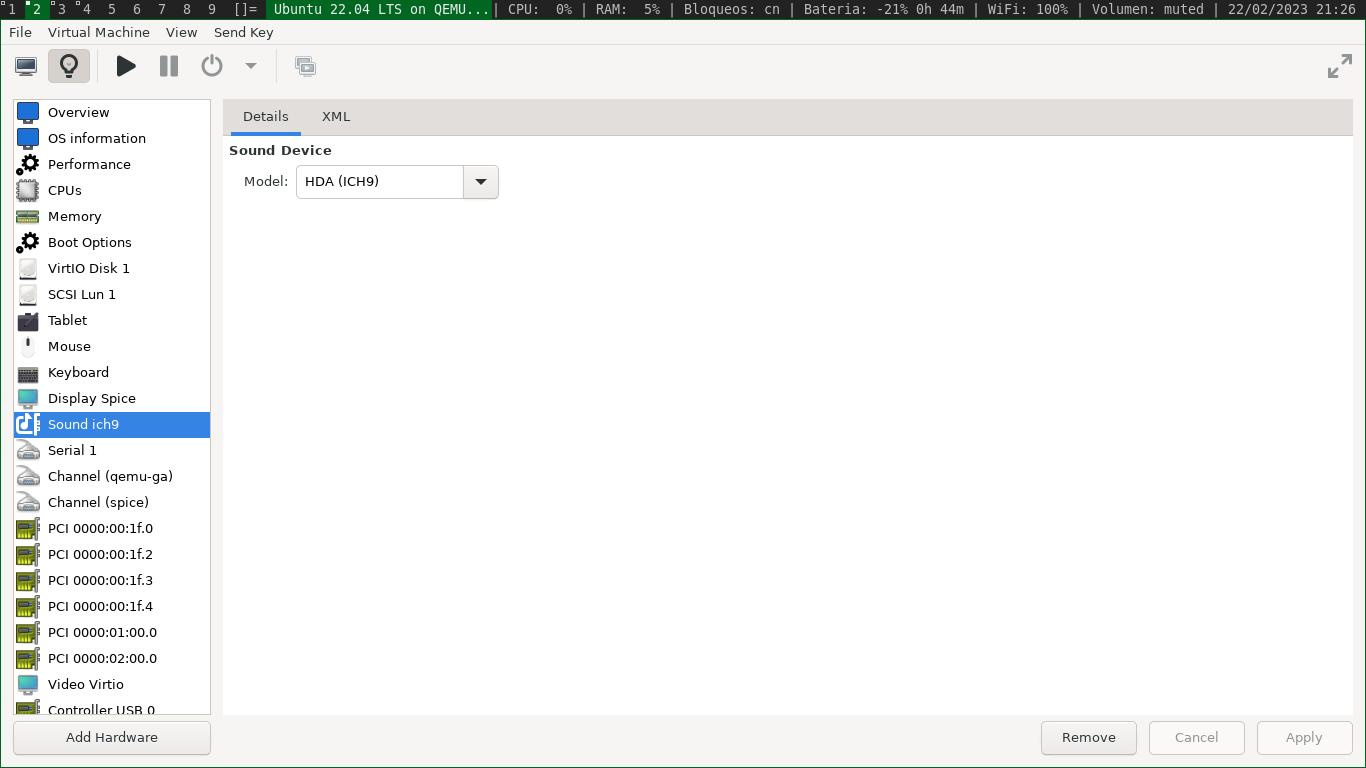
\includegraphics[width=\textwidth]{virtualMachine12}
\end{figure}
\newpage
\begin{figure}[!ht]
  \caption{Dispositivo Serial 1 de \acrshort{mv}}
  \centering
  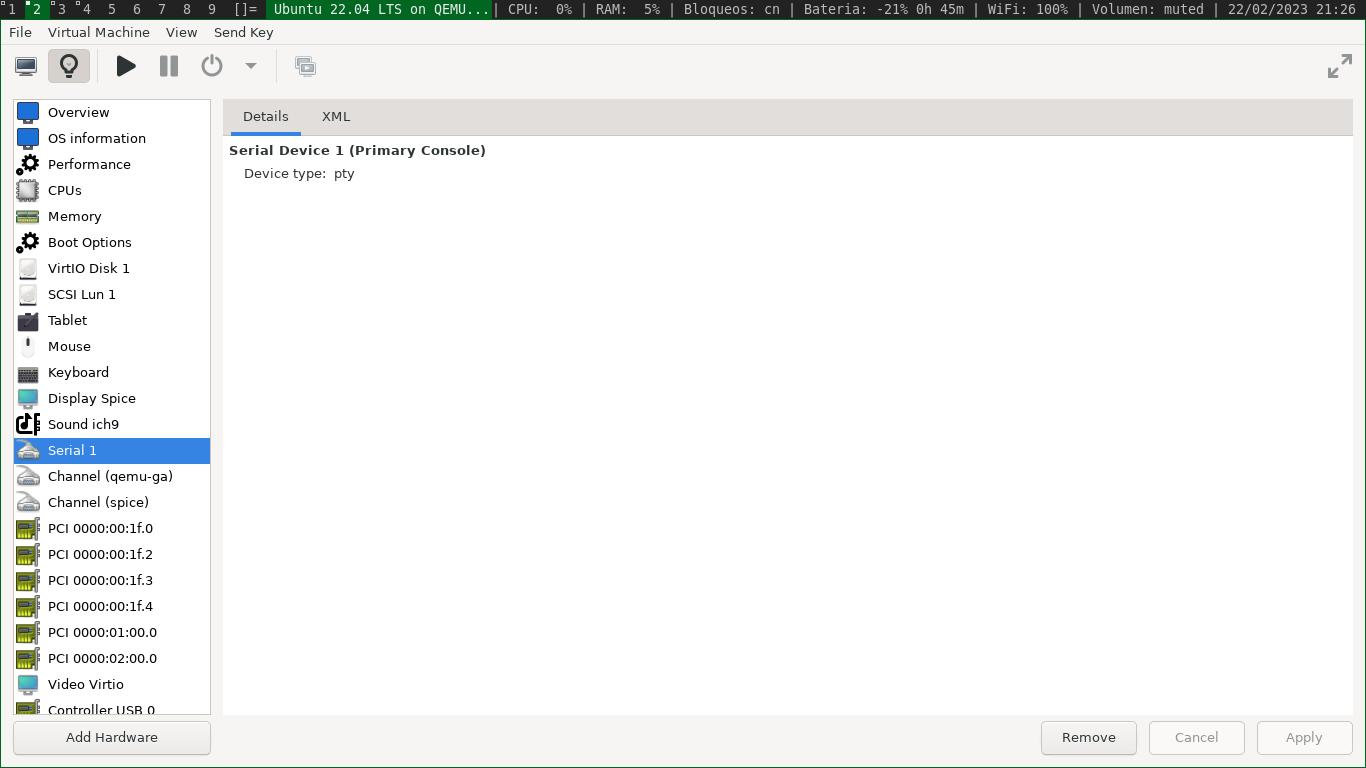
\includegraphics[width=\textwidth]{virtualMachine13}
\end{figure}
\begin{figure}[!ht]
  \caption{Canal qemu-ga de \acrshort{mv}}
  \centering
  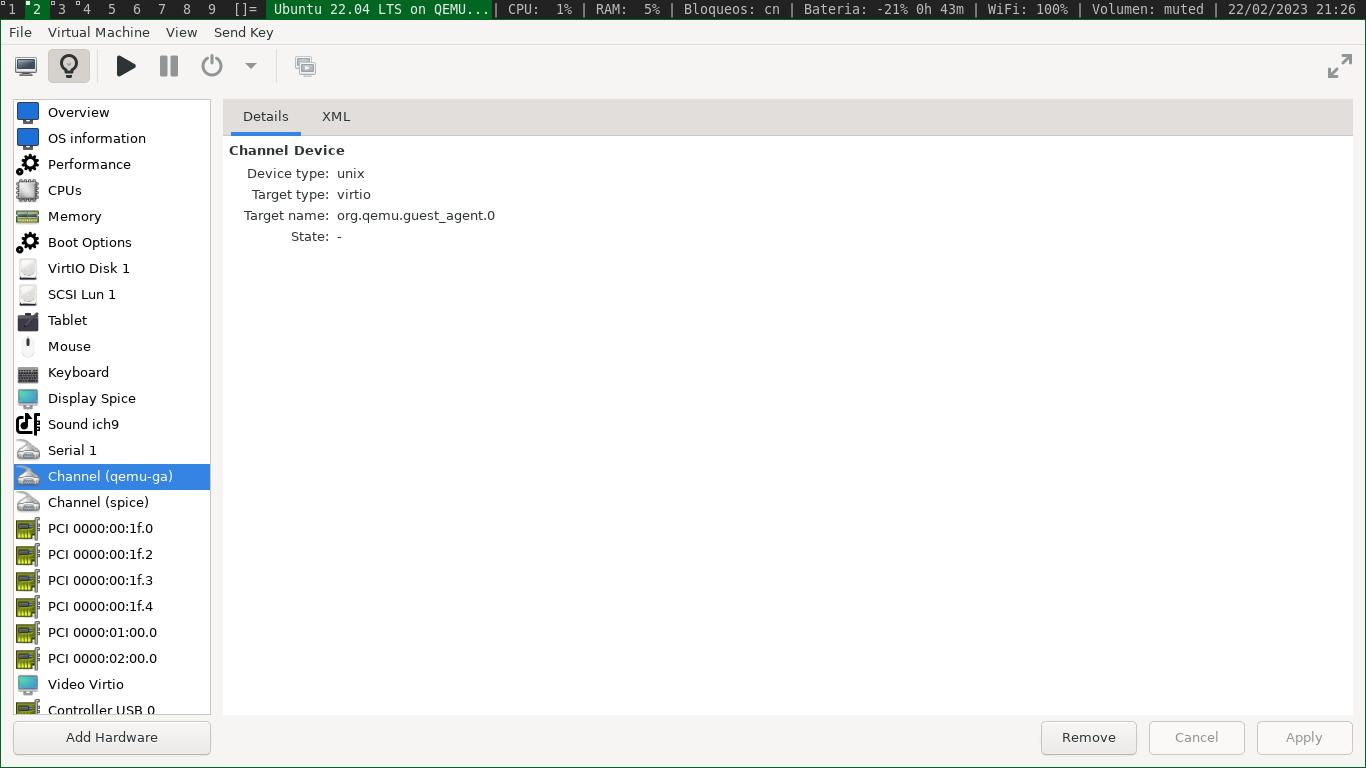
\includegraphics[width=\textwidth]{virtualMachine14}
\end{figure}
\newpage
\begin{figure}[!ht]
  \caption{Canal spice de \acrshort{mv}}
  \centering
  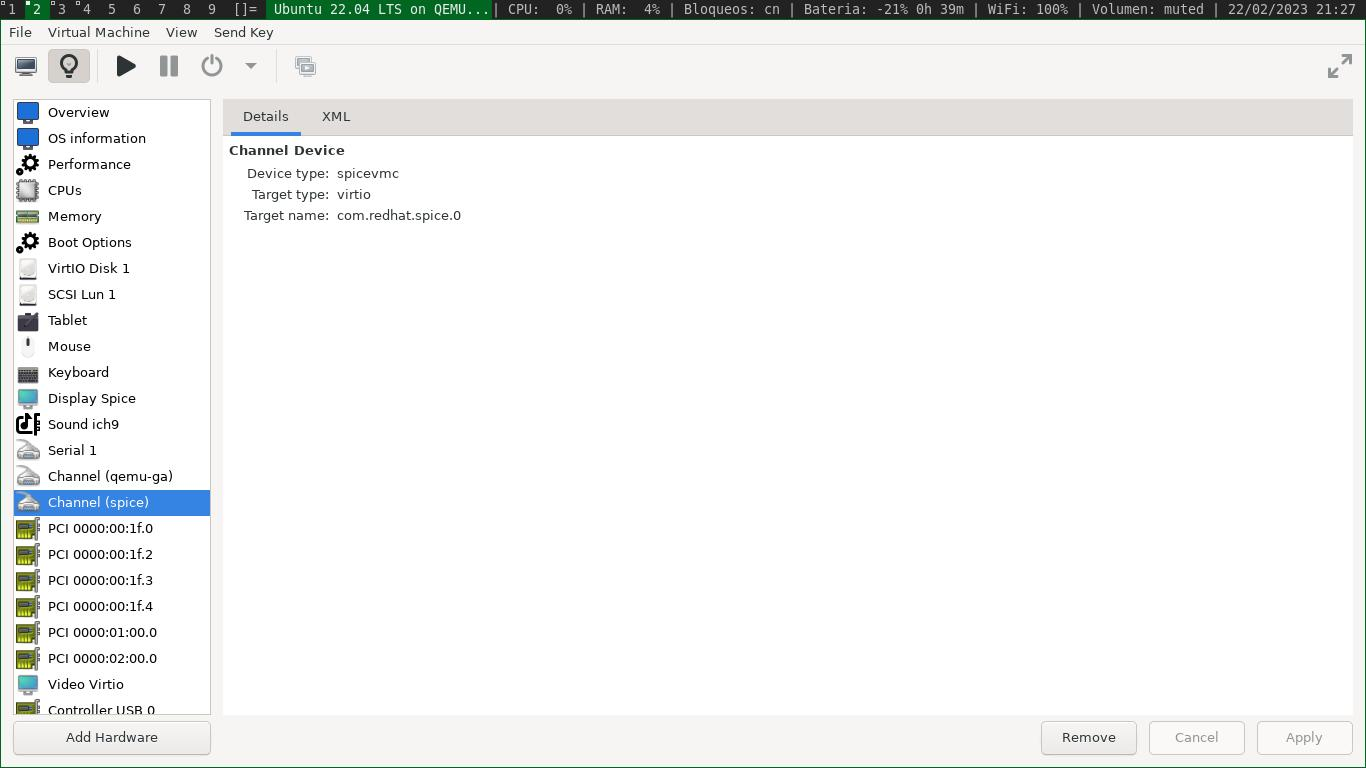
\includegraphics[width=\textwidth]{virtualMachine15}
\end{figure}
\begin{figure}[!ht]
  \caption{Controlador eSPI en \acrshort{mv}}
  \centering
  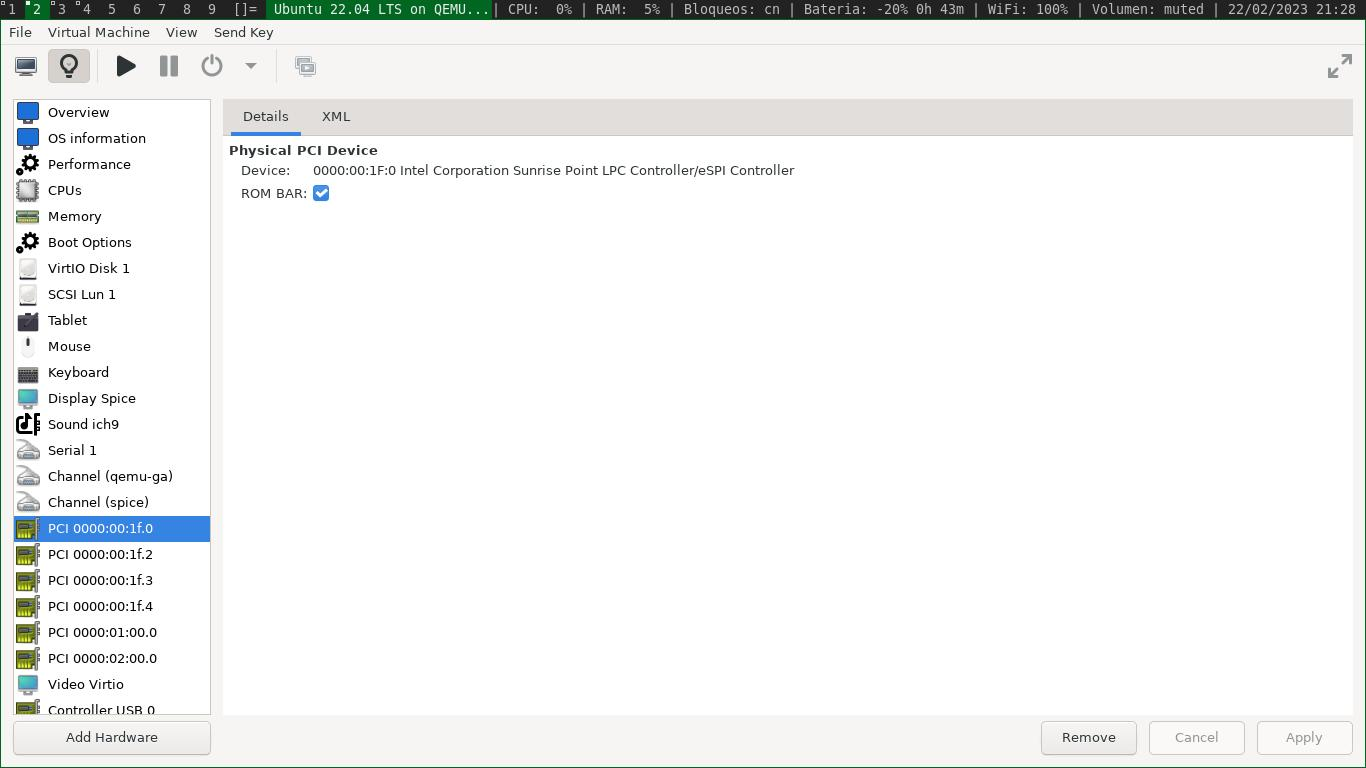
\includegraphics[width=\textwidth]{virtualMachine16}
\end{figure}
\newpage
\begin{figure}[!ht]
  \caption{Controlador de gestión de energía en \acrshort{mv}}
  \centering
  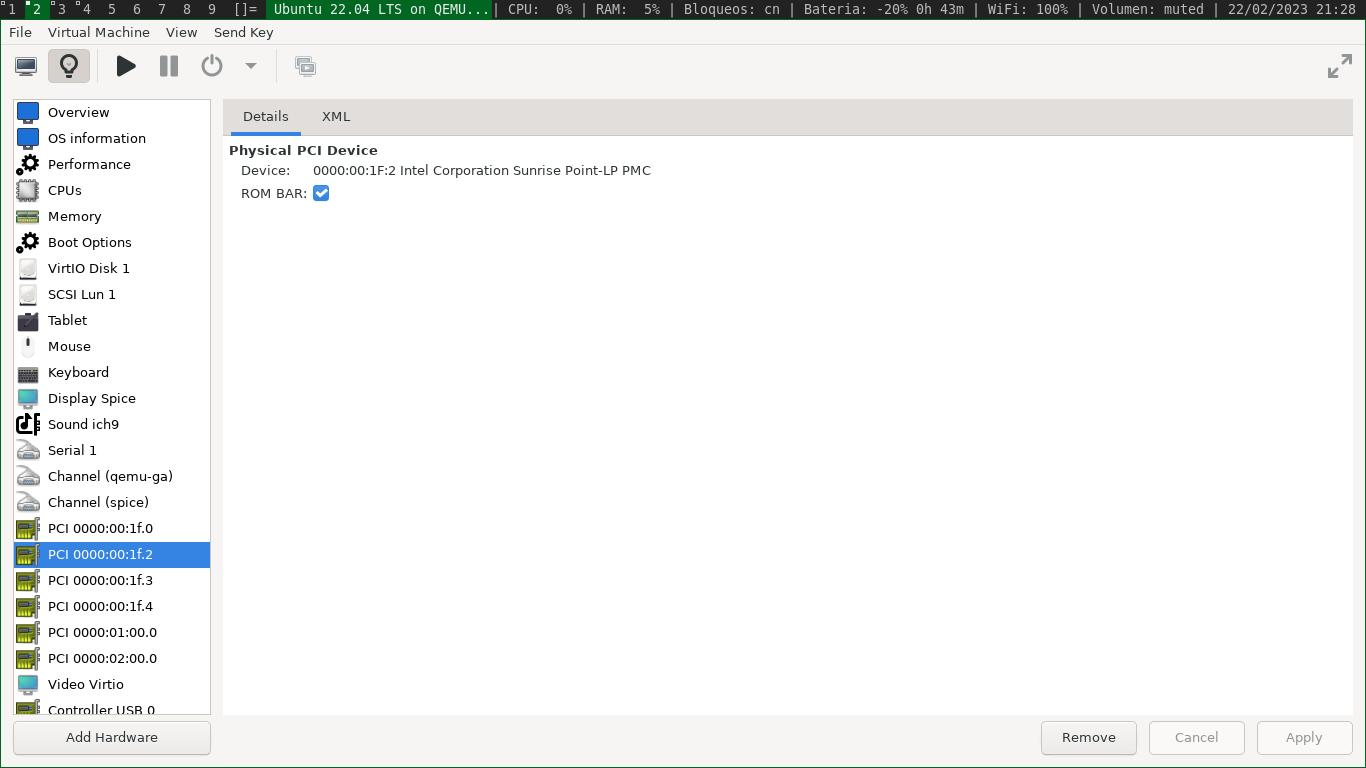
\includegraphics[width=\textwidth]{virtualMachine17}
\end{figure}
\begin{figure}[!ht]
  \caption{Controlador de Audio HD en \acrshort{mv}}
  \centering
  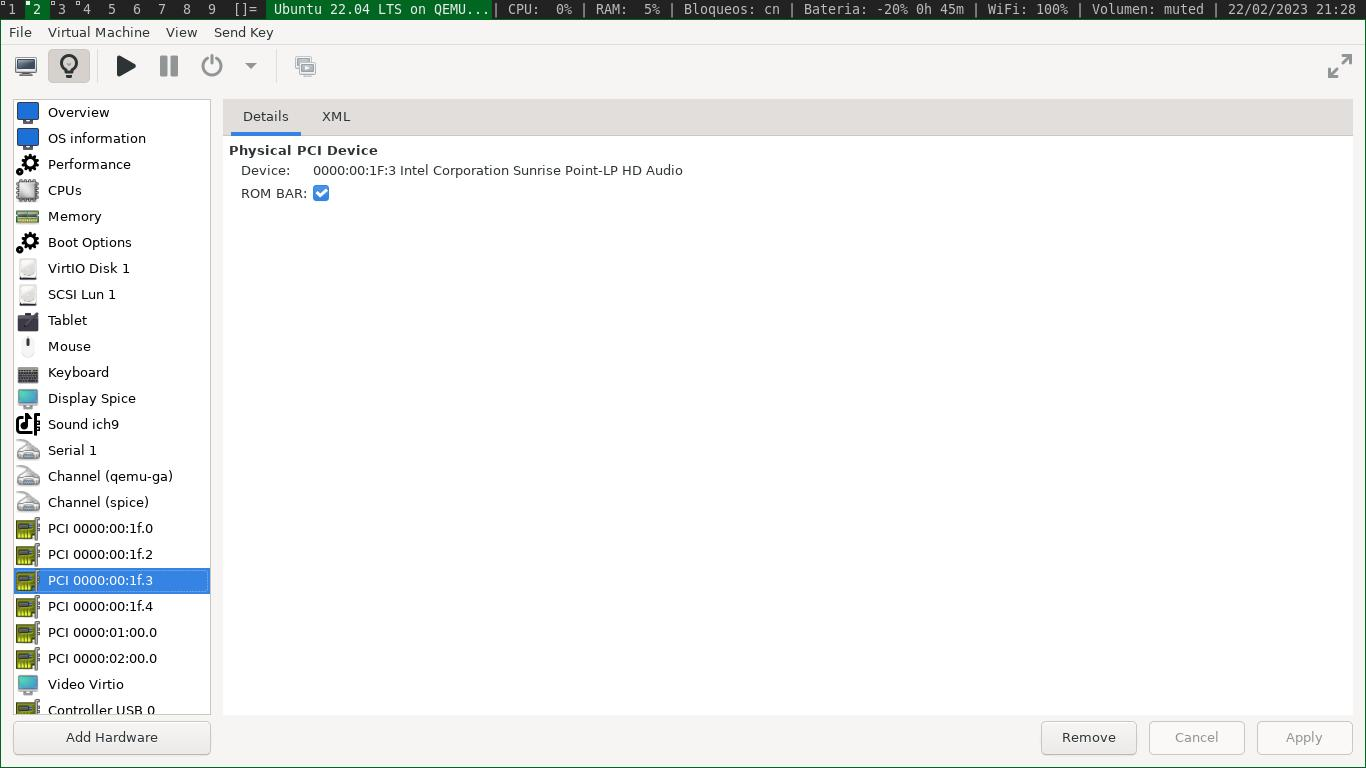
\includegraphics[width=\textwidth]{virtualMachine18}
\end{figure}
\newpage
\begin{figure}[!ht]
  \caption{Bus de gestión del sistema en \acrshort{mv}}
  \centering
  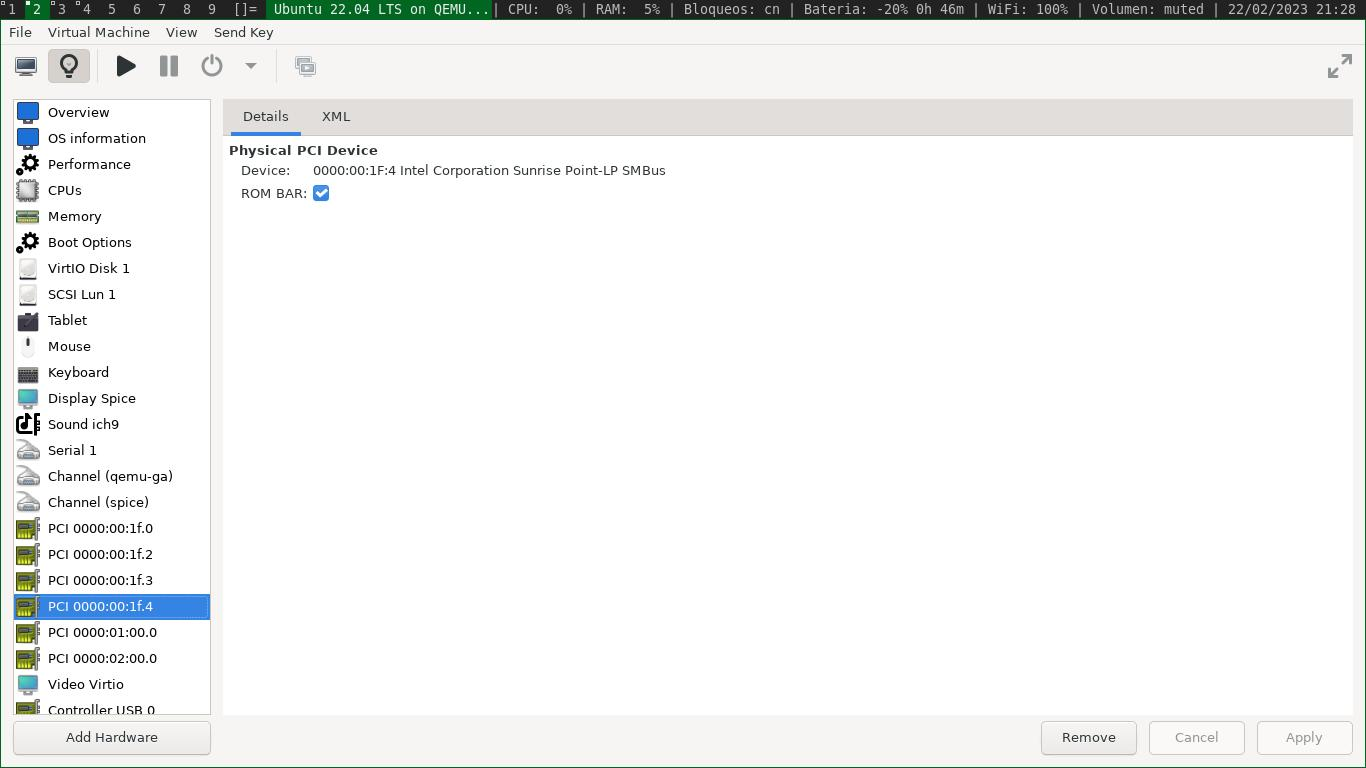
\includegraphics[width=\textwidth]{virtualMachine19}
\end{figure}
\begin{figure}[!ht]
  \caption{Controlador de Ethernet en \acrshort{mv}}
  \centering
  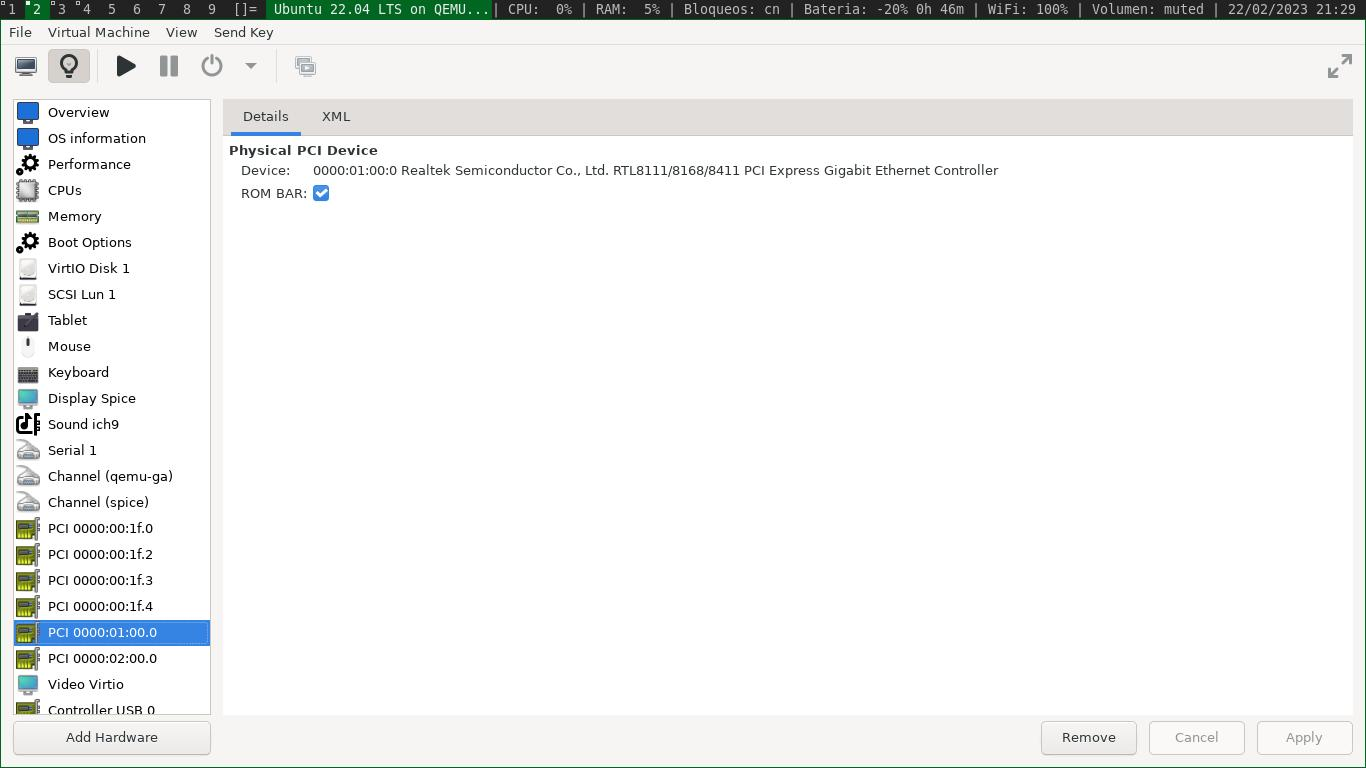
\includegraphics[width=\textwidth]{virtualMachine20}
\end{figure}
\newpage
\begin{figure}[!ht]
  \caption{Controlador de WiFi en \acrshort{mv}}
  \centering
  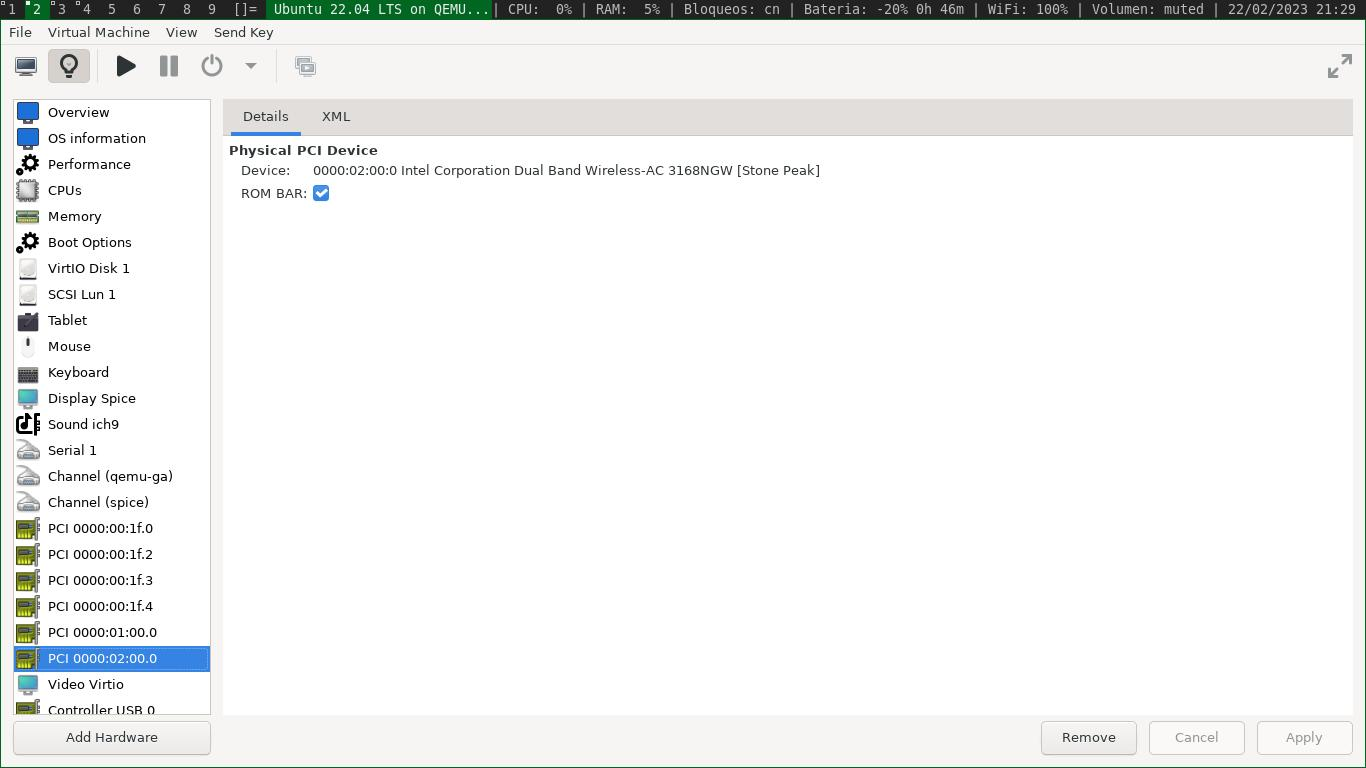
\includegraphics[width=\textwidth]{virtualMachine21}
\end{figure}
\begin{figure}[!ht]
  \caption{Modelo de video de \acrshort{mv}}
  \centering
  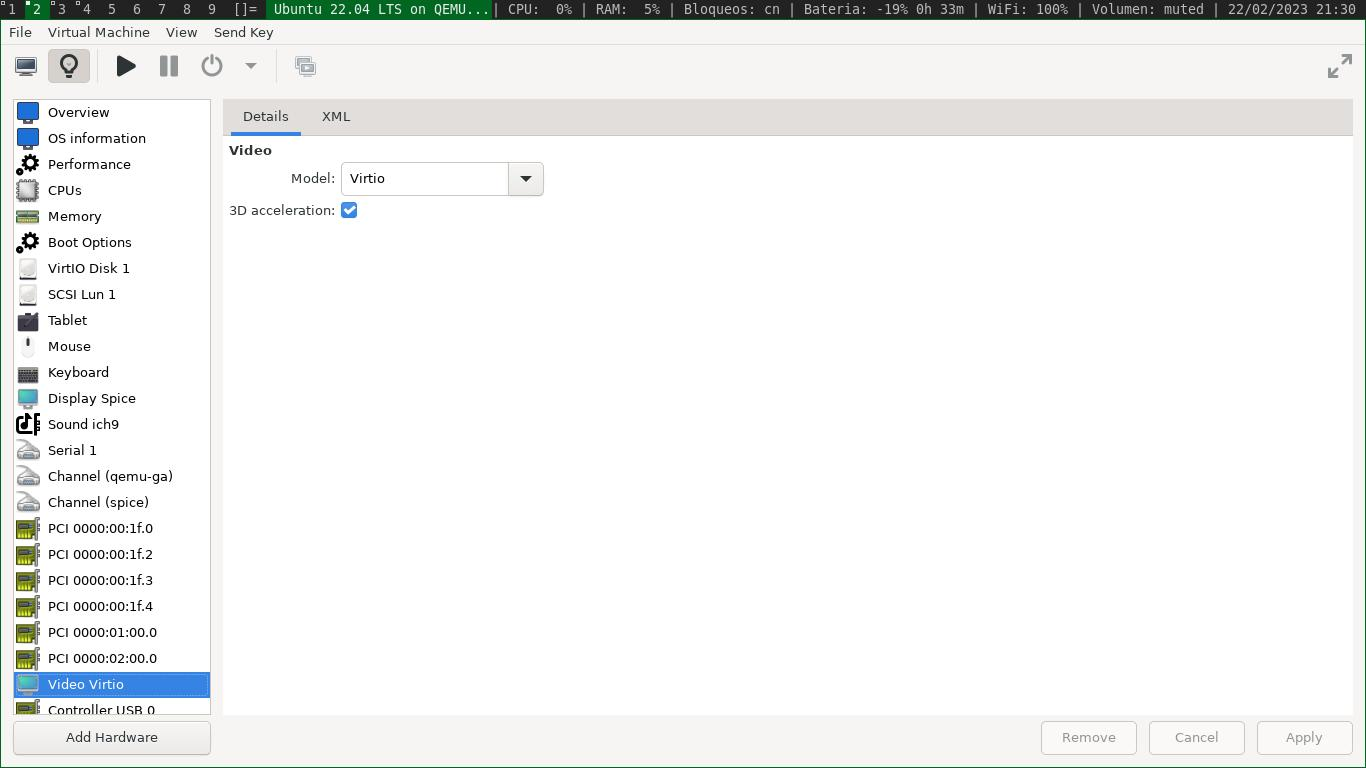
\includegraphics[width=\textwidth]{virtualMachine22}
\end{figure}
\newpage
\begin{figure}[!ht]
  \caption{Controlador USB de \acrshort{mv}}
  \centering
  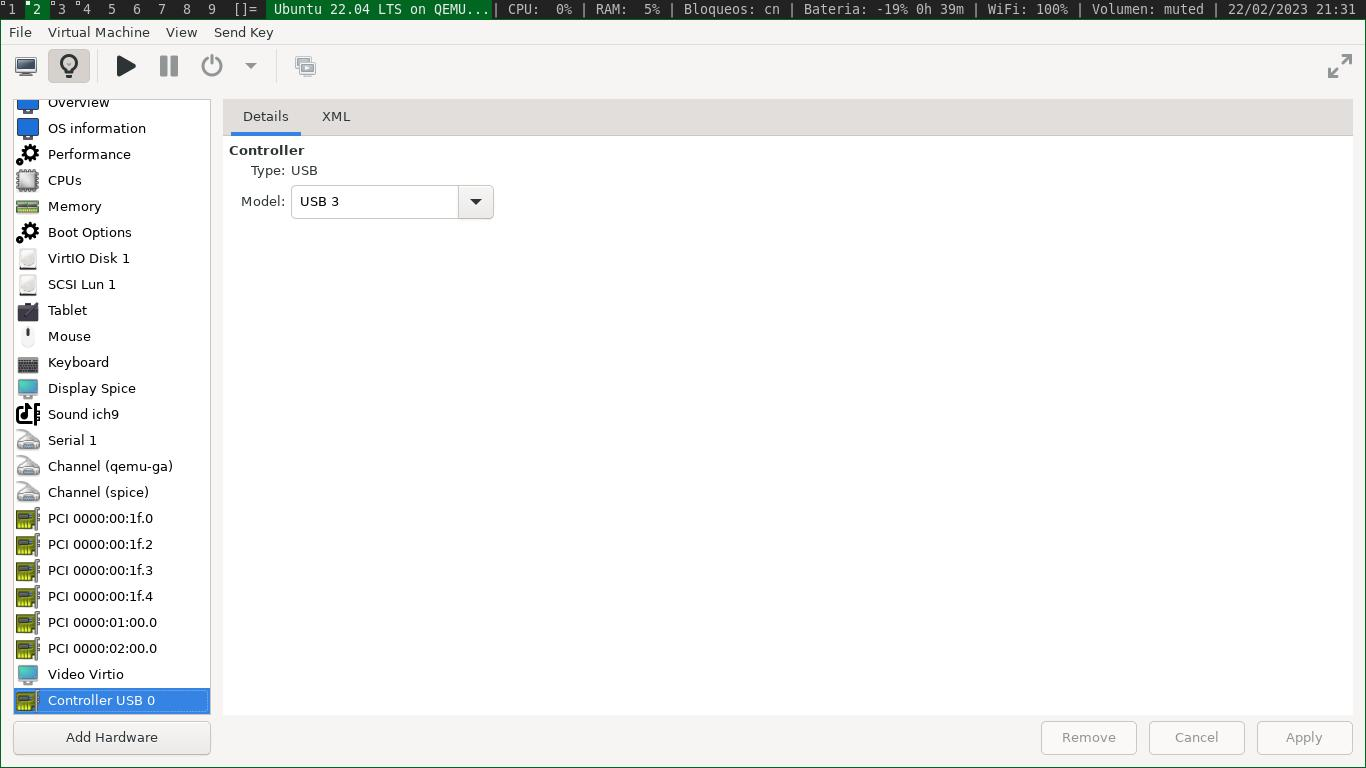
\includegraphics[width=\textwidth]{virtualMachine23}
\end{figure}
\begin{figure}[!ht]
  \caption{Controlador PCIe de \acrshort{mv}}
  \centering
  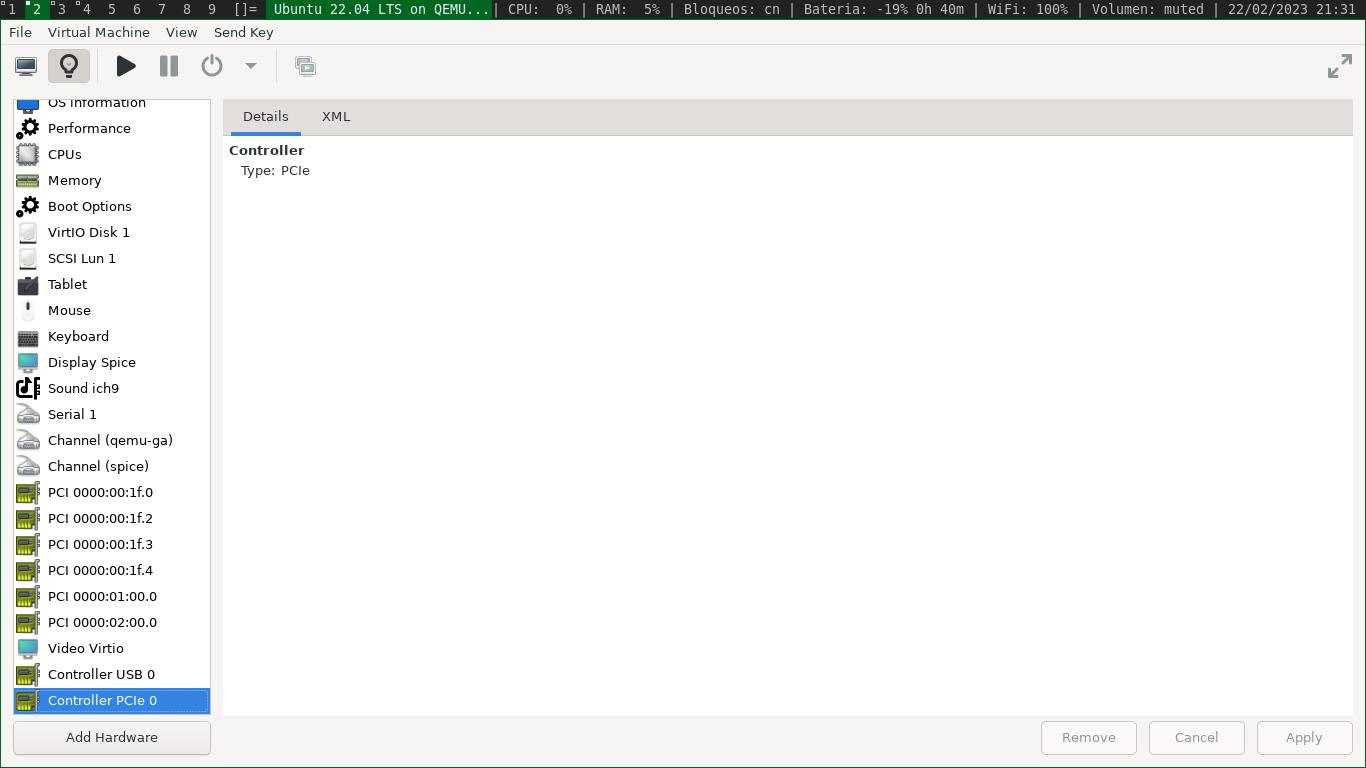
\includegraphics[width=\textwidth]{virtualMachine24}
\end{figure}
\newpage
\begin{figure}[!ht]
  \caption{Controlador PCI de \acrshort{mv}}
  \centering
  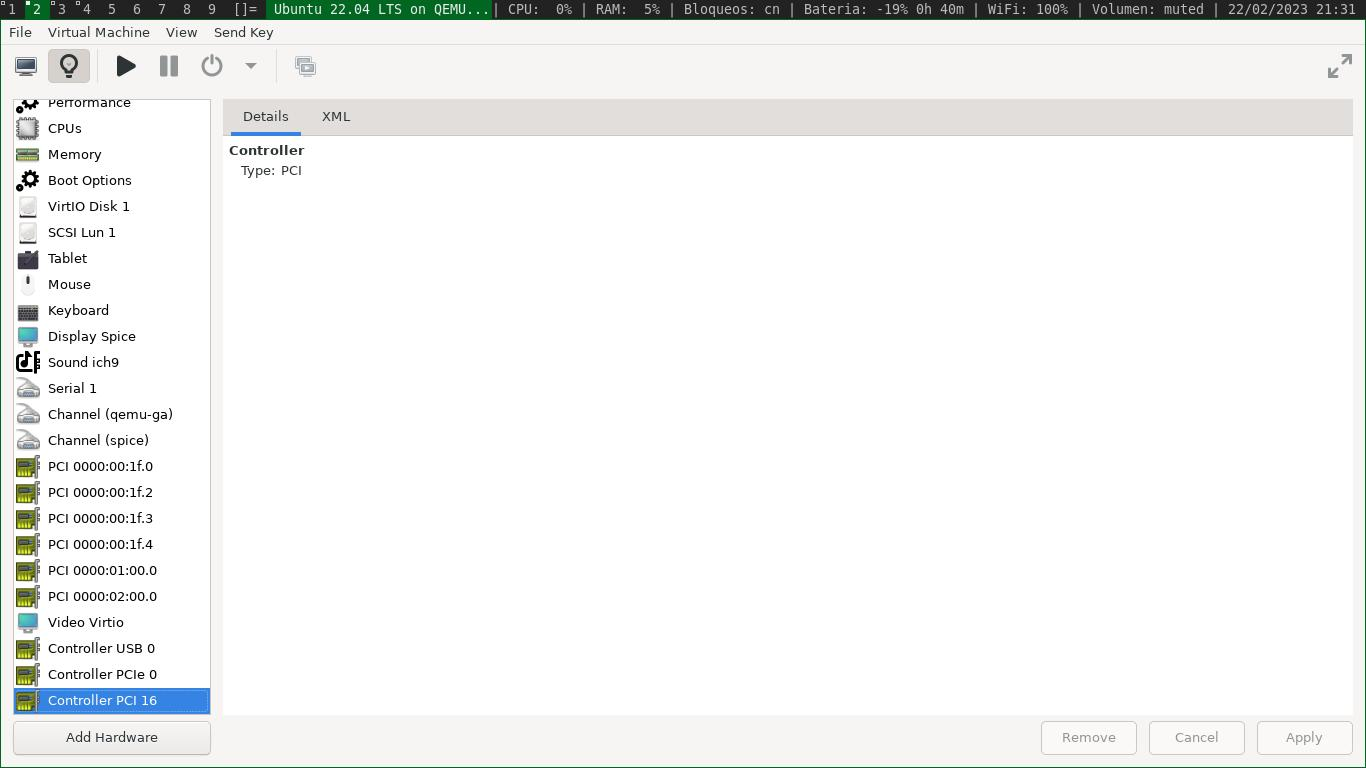
\includegraphics[width=\textwidth]{virtualMachine25}
\end{figure}
\begin{figure}[!ht]
  \caption{Controlador SATA de \acrshort{mv}}
  \centering
  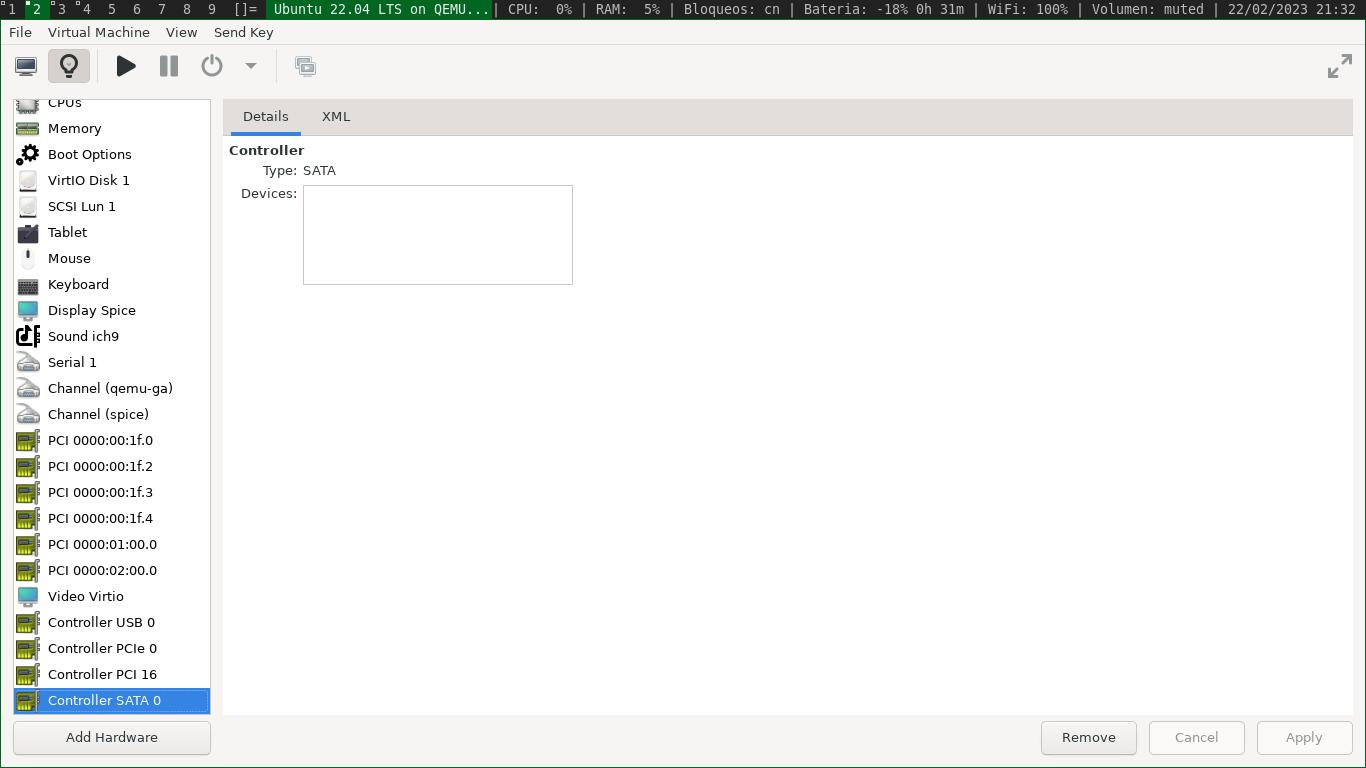
\includegraphics[width=\textwidth]{virtualMachine26}
\end{figure}
\newpage
\begin{figure}[!ht]
  \caption{Controlador Serial de \acrshort{mv}}
  \centering
  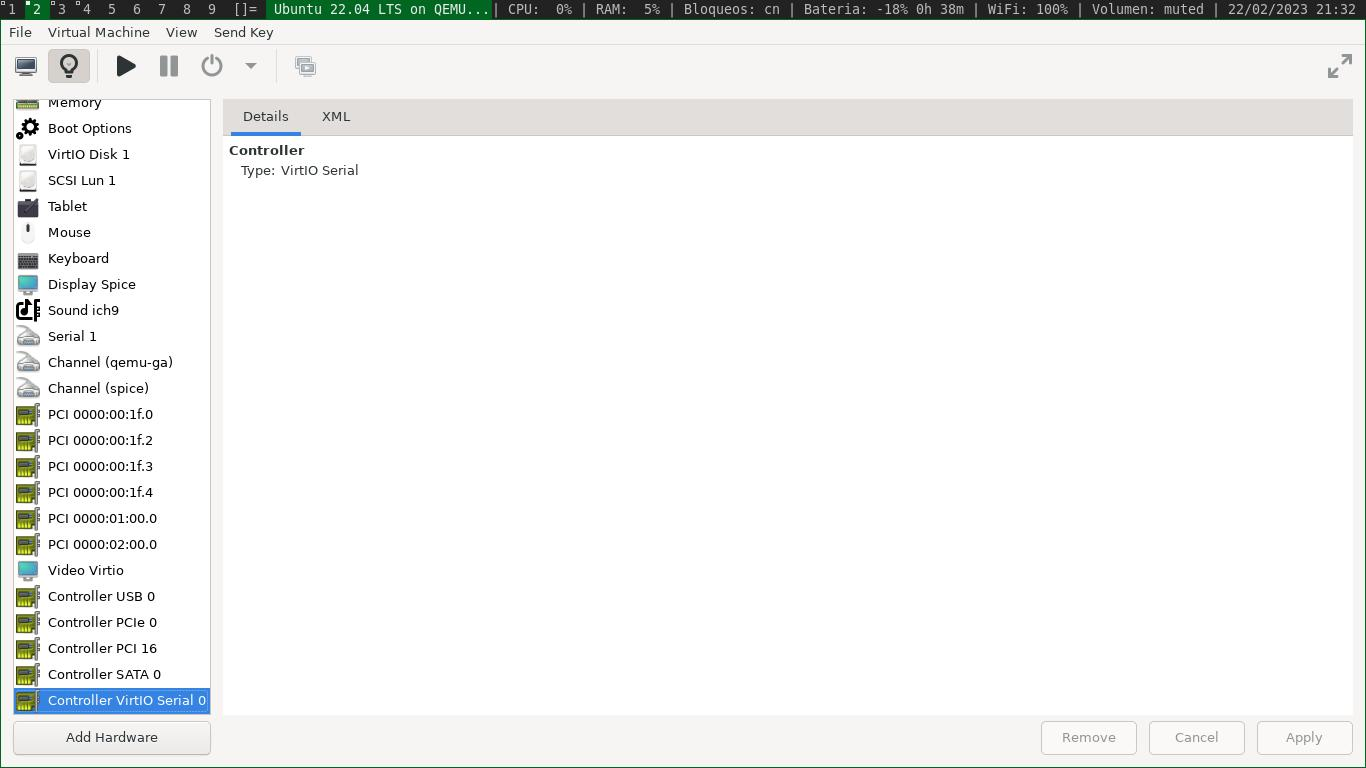
\includegraphics[width=\textwidth]{virtualMachine27}
\end{figure}
\begin{figure}[!ht]
  \caption{Controlador de lector de disco de \acrshort{mv}}
  \centering
  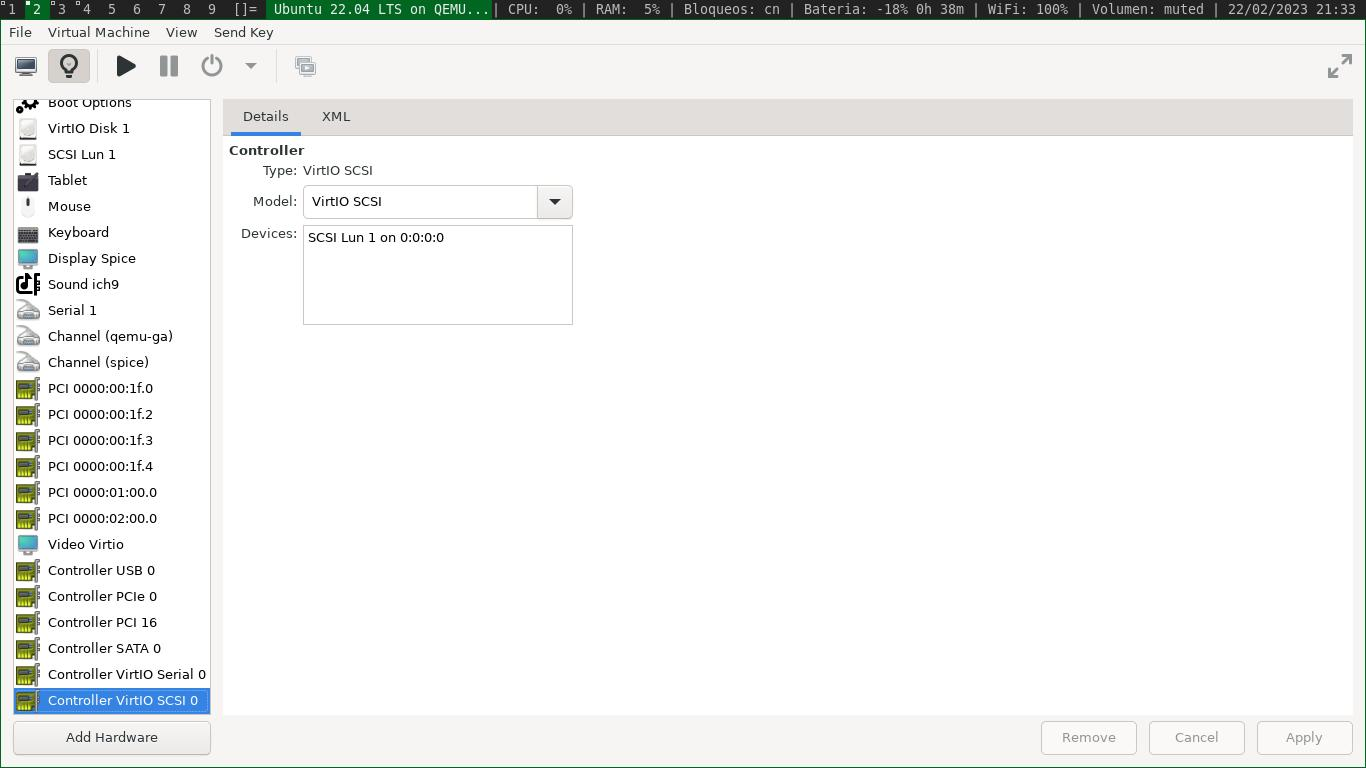
\includegraphics[width=\textwidth]{virtualMachine28}
\end{figure}
\newpage
\begin{figure}[!ht]
  \caption{Redoreccionador USB 1 de \acrshort{mv}}
  \centering
  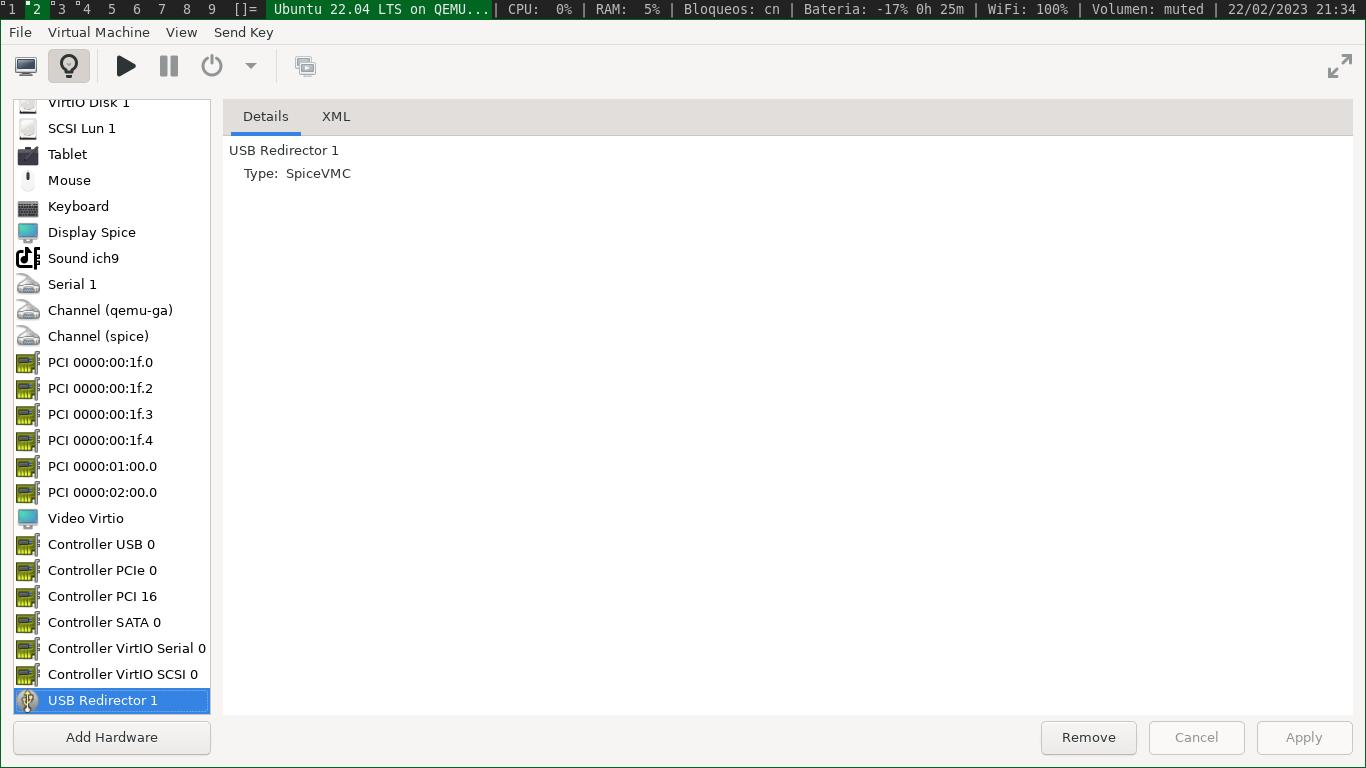
\includegraphics[width=\textwidth]{virtualMachine29}
\end{figure}
\begin{figure}[!ht]
  \caption{Redoreccionador USB 2 de \acrshort{mv}}
  \centering
  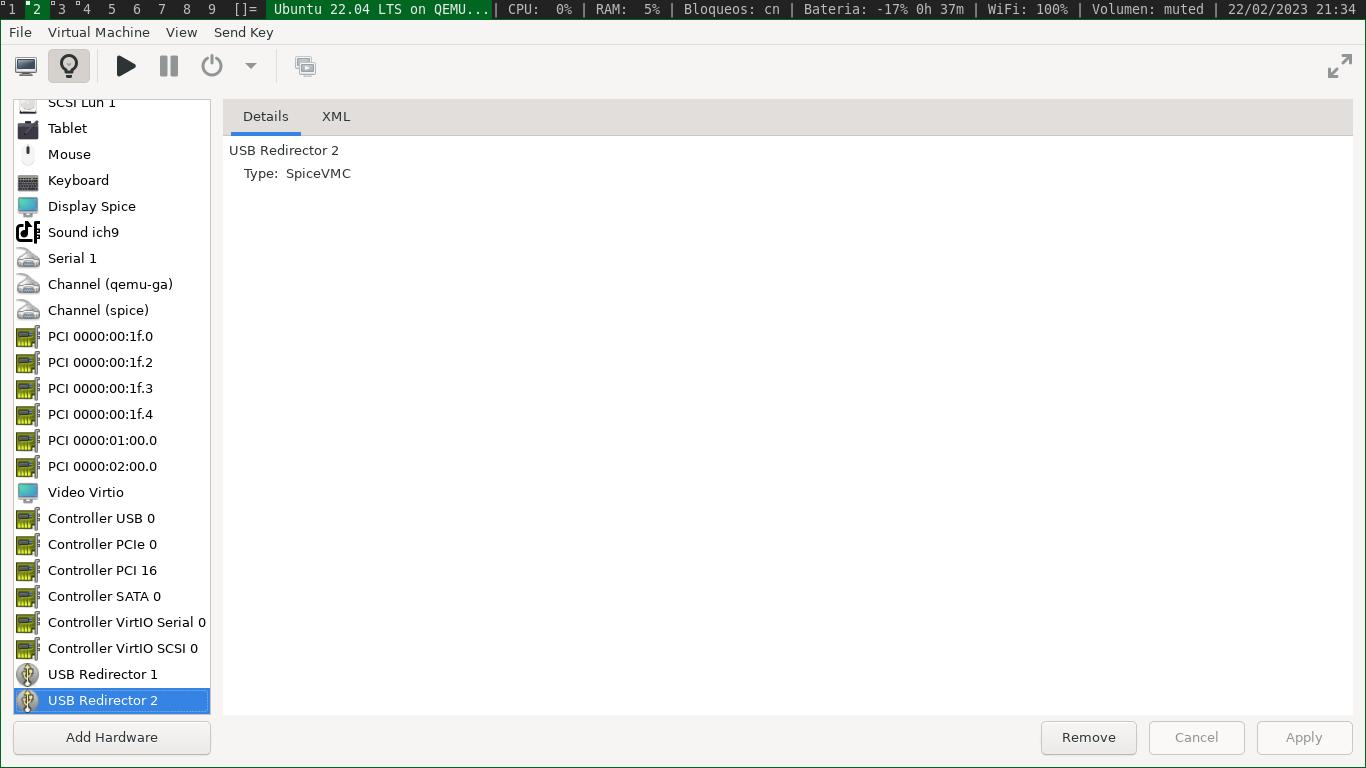
\includegraphics[width=\textwidth]{virtualMachine30}
\end{figure}
\newpage
\begin{figure}[!ht]
  \caption{Generador de números aleatorios de \acrshort{mv}}
  \centering
  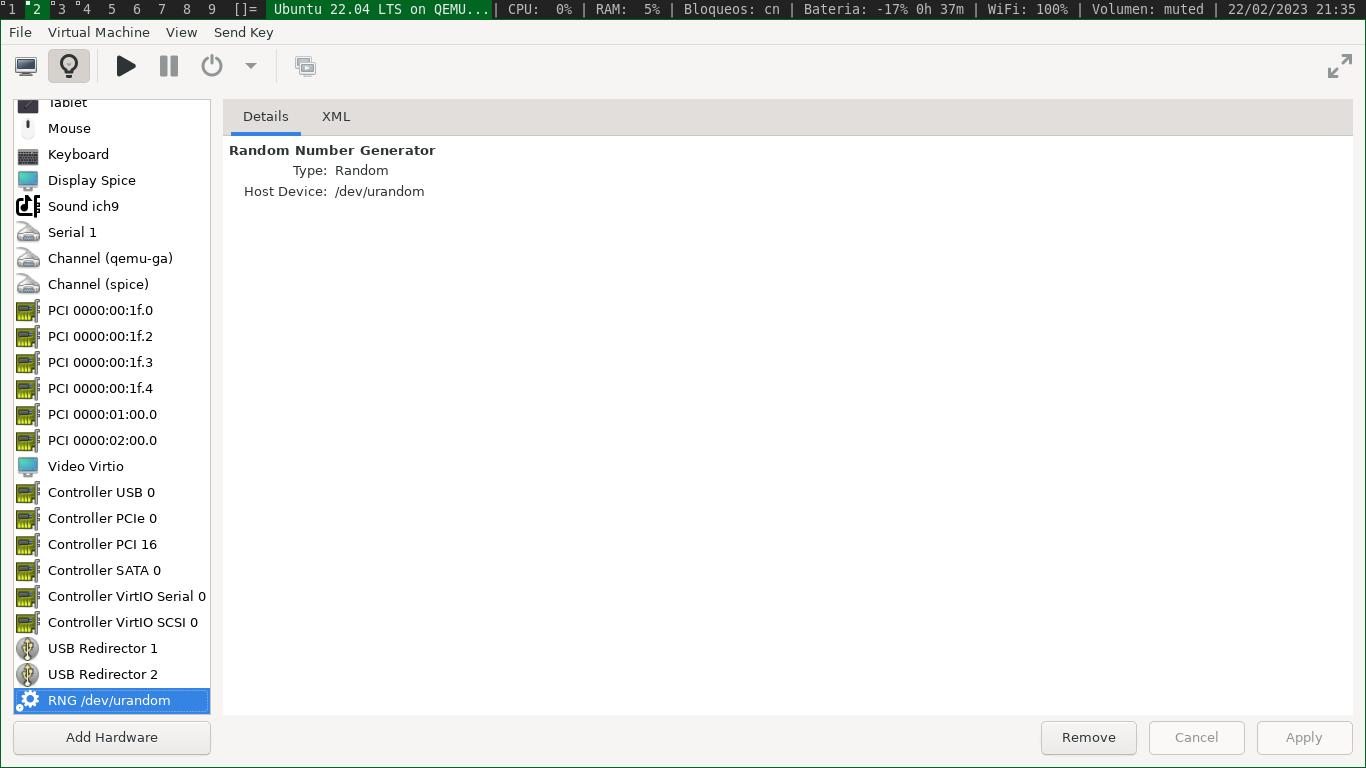
\includegraphics[width=\textwidth]{virtualMachine31}
\end{figure}
\normalsize{ \indent
Para la instalación de los paquetes de Haskell,
se utilizará el gestor de paquetes Apt; de todas
formas, es posible mejorar la experiencia de
ciertas características utilizando cabal (aunque
para lo que se realizará, no hará falta).
}
\newline
\normalsize{ \indent
Si bien, puede instalarse Termonad por el gestor
de paquetes; la única forma de que el programa
sea modificable con un archivo de Haskell es
compilando el programa (revisar
\url{https://github.com/cdepillabout/termonad#running-with-stack}),
por lo que se necesitará adicionalmente Stack
\cite{haskell_stack}.
}
